\par
In this chapter, I report the internship research I began at LBNL in the summer of 2022 that I have continued to work on as part of my doctoral studies.
We begin with elaborating more details of Figure~\ref{fig_rheology} from Chapter~\ref{sec:intro_complex_fluid}. 

\section{Rate-dependent flow}
In general, most non-Newtonian behaviors of complex fluids can be captured via shear rate dependency. 
We can describe rate-dependent flow with the following power law~\cite{herschel_konsistenzmessungen_1926}. We then have the viscous stress tensor, 
\begin{equation}
  {\bm \tau}
  =2^n \tilde{\mu} \dot{\gamma} ^{n-1} {\bm D},
  \label{eq_HS_tau}
  \end{equation}
where $\tilde{\mu}$ is the constant viscosity under zero shear rate and $n$ is the flow behavior index that can be determined experimentally depending on the materials.
We also recall that the magnitude of strain rate is $\dot{\gamma} = |\bm{D}|$.
Note that this value can be computed by applying the scaled Frobenius norm for a second-order tensor, 
\[
  \dot{\gamma}  = |\bm{D}| = \sqrt{\frac{1}{2}
    \text{tr}\left(\bm{D} \bm{D}^{T} \right)}.
\]
% In general, the Frobenius norm states $\bm{D}^H$ instead of $\bm{D}^T$. Since we consider real-valued tensors.
% Note that we return to the Newtonian fluid viscosity when $n = 1$, as introduced in equation (\ref{eq_stress_tensor}). 
% As we described in Figure~\ref{fig_rheology}, we see a shear-thinning fluid, also called pseudoplastic fluid, if 
\begin{figure}[ht]
  \begin{center}
    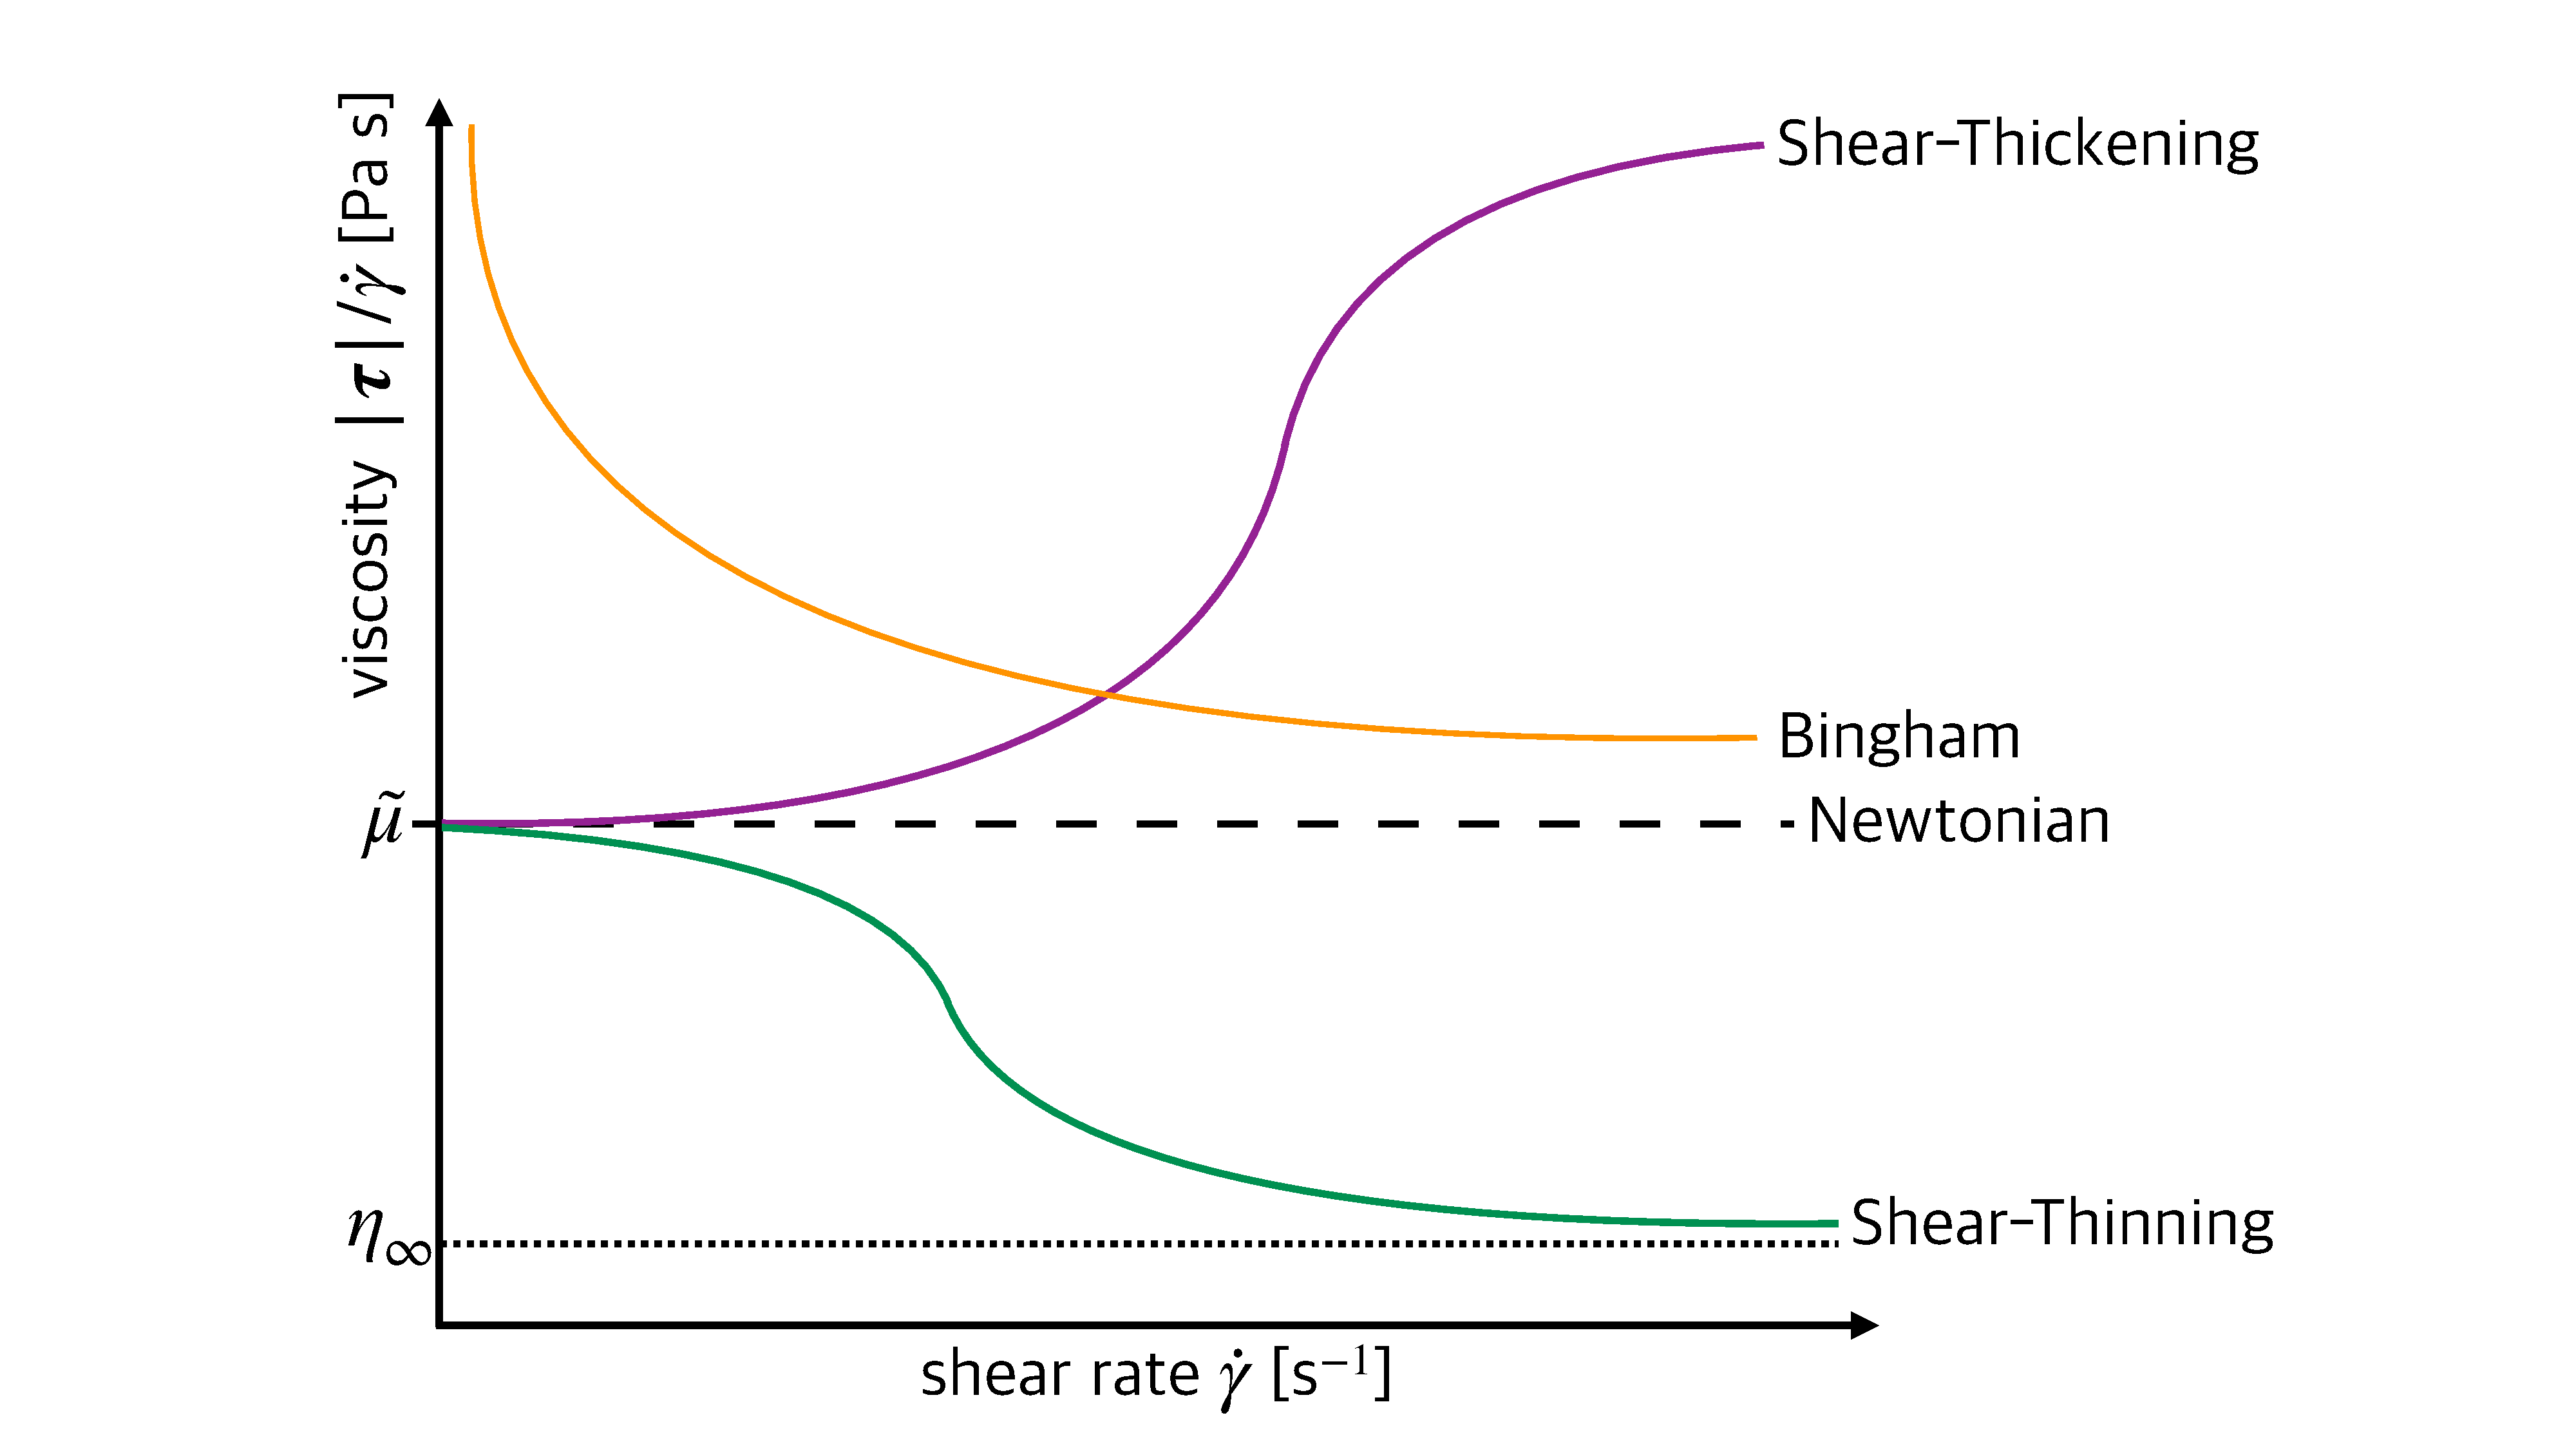
\includegraphics[scale=0.19]{figures/fig_appr_viscosity.pdf}
    \end{center}
  \caption{Relationship between apparent viscosity and shear rate. The plot is drawn based on~\cite{irgens_rheology_2014}. The value $\eta_{\infty}$ is the asymptotic viscosity at high shear rate.}
  \label{fig_appr_viscosity}
\end{figure}
\par
The relationship between rate-dependent flow and shear rate can be addressed with the \textit{apparent viscosity} function, $\eta$,
% To understand the relationship between rate-dependent flow and shear rate better, we introduce the function called \textit{apparent viscosity}, $\eta$,
\begin{equation}
  \eta(\dot{\gamma})
    =2^{n-1} \tilde{\mu} \dot{\gamma} ^{n-1}.
  \label{eq_appr_viscosity}
\end{equation}
We show the variation of apparent viscosity depending on the shear rate in Figure~\ref{fig_appr_viscosity}.
The black dashed line can be found when $n = 1$ in equation~(\ref{eq_appr_viscosity}) where the Newtonian fluid viscosity $\tilde{\mu}$ as introduced in equation (\ref{eq_stress_tensor}). 
% Note that $\eta_{\infty}$ is the asymptotic viscosity value at high shear rate.
Furthermore, the purple and green lines in Figure~\ref{fig_appr_viscosity} imply that the shear-thinning and thickening behaviors can be found when $n < 1$ and $n>1$, respectively. 
% We will discuss more of Bingham fluid and yield stress in the following section. 
% \subsection{Yield stress}
% The main characteristic of rate-dependent fluids is yield stress. 
\par
As we have shown in Figure~\ref{fig_rheology} in Chapter 1.3, a Bingham fluid is a particular case of the rate-dependent flow. 
Bingham fluid behaves as a solid, like plastic, under stress less than the yield stress and begins flowing like a fluid with varying viscosity. 
This is why it is classified as a \textit{viscoplastic} fluid.
The rheological equations describing Bingham fluid~\cite{bingham_investigation_1917} with yield stress $\tau_0$ are,
\begin{align}
  \left\{\begin{matrix}
 {\bm D} =0, & \text { if } |{\bm \tau} | <\tau_0 \\
  {\bm \tau}  = 
\left(2 \tilde{\mu} + \frac{\tau_0}{ \dot{\gamma}}\right) {\bm D} , & \text { if } |{\bm \tau}|\geq \tau_0,
\end{matrix}\right.
\label{eq_Bingham}
  \end{align}
and its corresponding apparent viscosity is
\begin{equation}
  \eta=\tilde{\mu} +\frac{\tau_0}{2 \dot{\gamma}},
  \end{equation}
  when $|\bm{\tau}| \geq \tau_0$.
  To illustrate more general yield stress fluids,~\cite{sverdrup_highly_2018} proposed the constitutive equations by combining equations~(\ref{eq_HS_tau}) and~(\ref{eq_Bingham}),
  \begin{equation}
    \left\{\begin{matrix}
  {\bm D }=0, 
    & \text { if } |{\bm \tau}| < \tau_0 
    \\
    {\bm \tau}  =
    \left(2^n \tilde{\mu} \dot{\gamma}^{n-1} + \frac{\tau_0}{ \dot{\gamma}}\right) {\bm D}, 
    & \text { if } |{\bm \tau}|  \geq \tau_0,
  \end{matrix}\right. 
  \label{eq_HS_B}
   \end{equation}
When $n = 1$, we recover the Bingham fluid.
% where $k$ is the consistency index, which is also determined by experiments along with the behavior index $n$, by measuring the fluid viscosity under the various shear rates, fitting the power law.
% A few examples of these indices $n$ and $k$ can be found in~\cite{irgens_rheology_2014}.
% \subsection{Viscosity regularization}
\par
As it is implied in equation~(\ref{eq_HS_B}), we obtain the yield stress of a fluid as $|\bm{\tau}| \rightarrow \tau_0$. 
When we solve for $\tau_0$ in equation~(\ref{eq_HS_B}), we see that 
\begin{equation}
2^n \tilde{\mu} \dot{\gamma}^{n} + \tau_0
\rightarrow \tau_0,
\end{equation}
due to $|\bm{D}| = \dot{\gamma}$, and thus, we should have 
\begin{equation}
  \dot{\gamma} \rightarrow 0.
\end{equation}
\par
Note that the computation of $\bm{\tau}$ is already implemented for a general rate-dependent fluid in AMReX. In the implementation, they use the Papanastasiou regularization method~\cite{papanastasiou_flows_1987}.
By introducing a small parameter, denoted as $\varepsilon$, we can regularize the singularity of $\dot{\gamma}$ as following,
\begin{equation}
  \frac{1}{\dot{\gamma}} \rightarrow \frac{1-e^{-\dot{\gamma} / \varepsilon}}{\dot{\gamma}}  
\end{equation}
for $\dot{\gamma}/\varepsilon \gg 1$. Otherwise, we simply use $1/\varepsilon$. 
The detailed mathematics and analysis can be found in~\cite{sverdrup_highly_2018}.



\section{Second-order strain rate rheolgy}
Once we obtain the stress tensor $\bm{\tau}$ for a complex fluid, we can incorporate the varying viscosity into the incompressible Navier-Stokes equations, which are introduced in~(\ref{eq_conserv_mass}) and~(\ref{eq_momentum_NS}), recalling here,
\begin{equation*}
  \nabla \cdot \vec{u} = 0 
  \nonumber
  % \label{eq_div_free} 
\end{equation*}
\begin{equation*}
  \frac{\partial \vec{u}}{\partial t} + \vec{u}\cdot \nabla \vec{u}
  = \frac{1}{\rho}
  \left(
  - \nabla P 
      + \nabla \cdot   \bm{\tau} 
      +  \rho  \vec{g} 
      \right),
      \nonumber
    % \label{eq_NS_ch4}
\end{equation*}
to obtain the flow velocity, $\vec{u}$.
\begin{comment}
To explain terminology, we write the stress tensor $\bar{\bar{\sigma}}$ explicitly, 
\begin{equation}
  \bar{\bar{\sigma}} = 
  \begin{bmatrix}
    \sigma_{xx} & \sigma_{xy} & \sigma_{xz} 
    \\
    \sigma_{xy} & \sigma_{yy} & \sigma_{zy} 
    \\
    \sigma_{xz} & \sigma_{zy} & \sigma_{zz}.
  \end{bmatrix}
  \label{eq_cauchy_mx}
\end{equation} 
Here, we define the first normal stress difference $N_1$
\begin{equation}
  N_1 = \sigma_{xx} - \sigma_{yy}
\end{equation}
and the second normal stress difference $N_2$,
\begin{equation}
  N_2 = \sigma_{yy} - \sigma_{zz}.
\end{equation}
the deviatoric stress tensor requires a higher-order relationship with the strain rate tensor $\bm{D}$. 
\end{comment}
We include a viscous stress tensor of the form,
\begin{equation}
   \boldsymbol{\tau} = 
   % 2 \nu_1  \bm{D} + 2 \nu_2  \bm{D}^2 ,
    \nu_0  \bm{A}_1 +  \nu_1  \bm{A}_1^2 + \nu_2 \bm{A}_2,
   \label{eq_CN_tau}
\end{equation}
where $\nu_0$ is constant in shear flow, and $\nu_1$ and $\nu_2$ are a function of the shear rate $\dot{\gamma}$.
The second-order form of the deviatoric stress tensor, equation~(\ref{eq_CN_tau}), was introduced by Colemann and Noll~\cite{coleman_approximation_1960}.
The term $\bm{A_i}$ is the Rivlin-Ericksen tensor, defined as
\begin{equation}
   {\bm A_1}  = \nabla \vec{u} +  \left( \nabla \vec{u} \right)^T = 2 \bm{D} 
   \label{eq_A1}
\end{equation}
and 
\begin{equation}
   \boldsymbol{A}_2
   % =\frac{D}{D t} \boldsymbol{A}_1+\boldsymbol{A}_1 \nabla \vec{u}+ \left(\nabla \vec{u} \right)^T \boldsymbol{A}_1
   =\frac{\partial \boldsymbol{A}_1}{\partial t} + \vec{u} \cdot \nabla \boldsymbol{A}_1+\boldsymbol{A}_1 \nabla \vec{u}+ \left(\nabla \vec{u} \right)^T \boldsymbol{A}_1.
   \label{eq_A2}
\end{equation}
Note that the general form of the Rivlin-Ericksen tensor can be extended to order $n$,  
\begin{equation}
  \boldsymbol{A}_{n+1}
  =\frac{\partial \boldsymbol{A}_{n}}{\partial t} + \vec{u} \cdot \nabla \boldsymbol{A}_n+\boldsymbol{A}_n \nabla \vec{u}+ \left(\nabla \vec{u} \right)^T \boldsymbol{A}_n.
\end{equation}
\par
For polymer solutions, the most studied in non-Newtonian fluids, it is well-known that the effect of the $\mathcal{O}\left( \bm{D}^2 \right)$ term is small enough to ignore, compared to  $\mathcal{O}\left( \bm{D} \right)$~\cite{bird_dynamics_1987}. For this reason, the effect of $\mathcal{O}\left( \bm{D}^2 \right)$ has been neglected in many research works for a complex fluid. 
For other materials, however, there are potentially important characteristics we should pay attention to considering the stress with higher-order terms in $\boldsymbol{D}$, including granular materials. 
As a first step, we thus explore the second-order rheology with granular materials.

% We will explore both first- and second-order rheologies, depending on the materials we consider. 
% In the following four sections, we discuss the viscous tensor term $\bm \tau$ for each type of complex fluid. 


\begin{comment}
\section{Second-order strain rate rheolgy}
We now consider the second-order strain rate term as introduced in~(\ref{eq_A2}), as well as the first-order term~(\ref{eq_A1}).
Examples included the suspension flow from Guazelli and the rod-climbing effect. The coefficients $\nu_0$ in the general form of the Rivlin-Ericksen tensor can be obtained by some formulae. 


We consider
\[
\vec{u}= (u, \ v, \ w)
\]
\[
\nabla \vec{u}
= 
\begin{bmatrix}
u_x & u_y & u_z
\\
v_x & v_y & v_z
\\
w_x & w_y & w_z
\end{bmatrix}
\]
We want to compute
\[
{\bm D} = \nabla \vec{u} + \left( \nabla \vec{u} \right)^T
\]


Let's see what $\bm{D}^2 = \left[D^2_1, \ D^2_2, \ D^2_3 \right]$ looks like first: 
\\
First column 
\[
D^2_1 = 
\begin{bmatrix}
 \left(u_y+v_x\right)^2+\left(u_z+w_x\right)^2+4 u_x^2 
 \\
  \left(u_z+w_x\right) \left(v_z+w_y\right)+2 \left(u_x+v_y\right) \left(u_y+v_x\right)
  \\
  \left(u_y+v_x\right) \left(v_z+w_y\right)+2 \left(u_x+w_z\right) \left(u_z+w_x\right)
\end{bmatrix}
\]
Second column
\[
D^2_2 = 
\begin{bmatrix}
 \left(u_z+w_x\right) \left(v_z+w_y\right)+2 \left(u_x+v_y\right) \left(u_y+v_x\right)
 \\
 \left(u_y+v_x\right)^2+\left(v_z+w_y\right)^2+4 v_y^2
 \\
 \left(u_y+v_x\right) \left(u_z+w_x\right)+2 \left(v_y+w_z\right) \left(v_z+w_y\right)
\end{bmatrix}
\]
Third column
\[
D^2_3=
\begin{bmatrix}
 \left(u_y+v_x\right) \left(v_z+w_y\right)+2 \left(u_x+w_z\right) \left(u_z+w_x\right)
 \\
 \left(u_y+v_x\right) \left(u_z+w_x\right)+2 \left(v_y+w_z\right) \left(v_z+w_y\right)
 \\
 \left(u_z+w_x\right)^2+\left(v_z+w_y\right)^2+4 w_z^2
\end{bmatrix}
\]
\end{comment}
\section{Granular rheology}
We model a new stress tensor $\bm \tau$ with a second-order strain rate that describes non-isotropic material flow properties,
\begin{align}
  \bar{\bar{\sigma}}
    = -P \bar{\bar{I}}  + \bm{\tau}
    =  -P \bar{\bar{I}}  
    + \mu_1(\dot{\gamma}) \mathcal{O}({\bm D})
    + \mu_2(\dot{\gamma}) \mathcal{O}({\bm D^2}).
  \end{align}
In this section, we focus on the methodology to compute the viscosity $\mu_i ({\dot{\gamma}})$ ($i = 1,2$) under the simple shear flow. 
% A new apparent viscosity computation using the well-known $\mu(I)$ relation can also be found [{\color{blue}REFERENCE}]. 
In~\cite{srivastava_viscometric_2021}, a new stress tensor is presented to describe a non-isotropic flow as follows,
%  of the form~(\ref{eq_CN_tau}), 
% \begin{align*}
% \bar{\bar{\sigma}} - P {\bm I} \equiv
%   {\bm {\bm \tau}}
%   =  \ \mu_1 {\bm D} 
%   + \mu_2  \left[ {\bm D}^2  - \frac{\text{tr}\left({\bm D}^2\right)}{3}{\bm I} \right]
%   + \eta_3  \left[ {\bm D}{\bm W} - {\bm W}{\bm D} \right]
%   \nonumber \\
%   + \frac{\kappa_1}{\dot{\gamma }^2} \bm D 
%   + \frac{\kappa_2}{\dot{\gamma }^2}  \left[ {\bm D}^2  
%   - \frac{\text{tr}\left({\bm D}^2\right)}{3}{\bm I} \right],
% \end{align*}
\begin{equation}
  {\bm {\bm \tau}}
  = \mu_1(\dot{\gamma}) {\bm D}
  +  
 \mu_2 (\dot{\gamma})
  \left[ {\bm D}^2  - \frac{\text{tr}\left({\bm D}^2\right)}{3}{\bm I} \right],
  % \ + \
  % \left( \mu_3 \dot{\gamma}^2 \right)
  % \frac{1}{\dot{\gamma}^2}
  %   \left[ {\bm D}{\bm W} - {\bm W}{\bm D} \right]
\label{eq_2ndOrder_tau}
\end{equation}
where 
\begin{equation}
  \mu_1 (\dot{\gamma})
   = \left( \eta_1 \dot{\gamma}+ \kappa_1 \right) \frac{1}{\dot{\gamma}},
\label{eq_mu1_main}
\end{equation}
and 
\begin{equation}
  \mu_2 (\dot{\gamma}) = 
  \left( \eta_2  \dot{\gamma}^2
  +  \kappa_2 
  \right) \frac{1}{\dot{\gamma}^2}.
  \label{eq_mu2_main}
\end{equation}
As a particular application to equation~(\ref{eq_CN_tau}), the form~(\ref{eq_mu2_main}) is derived under two conditions:
(1) the flow motion is simple with a constant stretch by neglecting deformation history, and (2) the flow is isochoric, having uniform properties along streamlines and tr$(D) = 0$. 
Note that the last term in equation~(\ref{eq_2ndOrder_tau}) with tr$\left( \bm D^2 \right)$ appears to show the pressure dependency of the granular material, in addition to the hydrostatic pressure $P$~\cite{rajagopal_implicit_2006}.



% In particular, we see \cite{srivastava_viscometric_2021}


% it is valid to have $\bm{D}^H = \bm{D}^T$.
\par
The flow functions, $\eta_i$ and $\kappa_i$ for $i = 1,2$, have the following dependence on total stress: each $\eta_i(\dot{\gamma}, p)$ is (shear) rate-dependent and $\kappa_i (p)$ is (shear) rate-independent. 
% Along with the shear effect from $\eta_1$, we can observe the second normal-stress difference in shear flows from $\eta_2$.
% The rate-independent terms, $\kappa_1$ and $\kappa_2$, allow us to find yield stress. 
We shall explain the details of these two types of functions in the following sub-section.

\subsection{$\mu (I)$ rheology}
The key to modeling the $\eta_i$ and $\kappa_i$ terms is the well-known $\mu(I)$ relationship developed by~\cite{jop_constitutive_2006}.
Here, $I$ is the \textit{inertial number},
\begin{equation}
  I =  \frac{\dot{\gamma} d }{\sqrt{P/\rho_p}},
  \label{eq_inertialI}
\end{equation}
where $d$ and $\rho_p$ are the average particle diameter and density of a given granular material.
This dimensionless quantity describes the ratio of the average static force to the inertial force between granular particles,~\cite{jop_constitutive_2006} interpreted the inertial number as the ratio between a macroscopic deformation and an inertial timescale. 
\par
To understand the granular flow regimes depending on the inertial number. We consider an hourglass example. 
\begin{figure}[ht]
  \begin{center}
    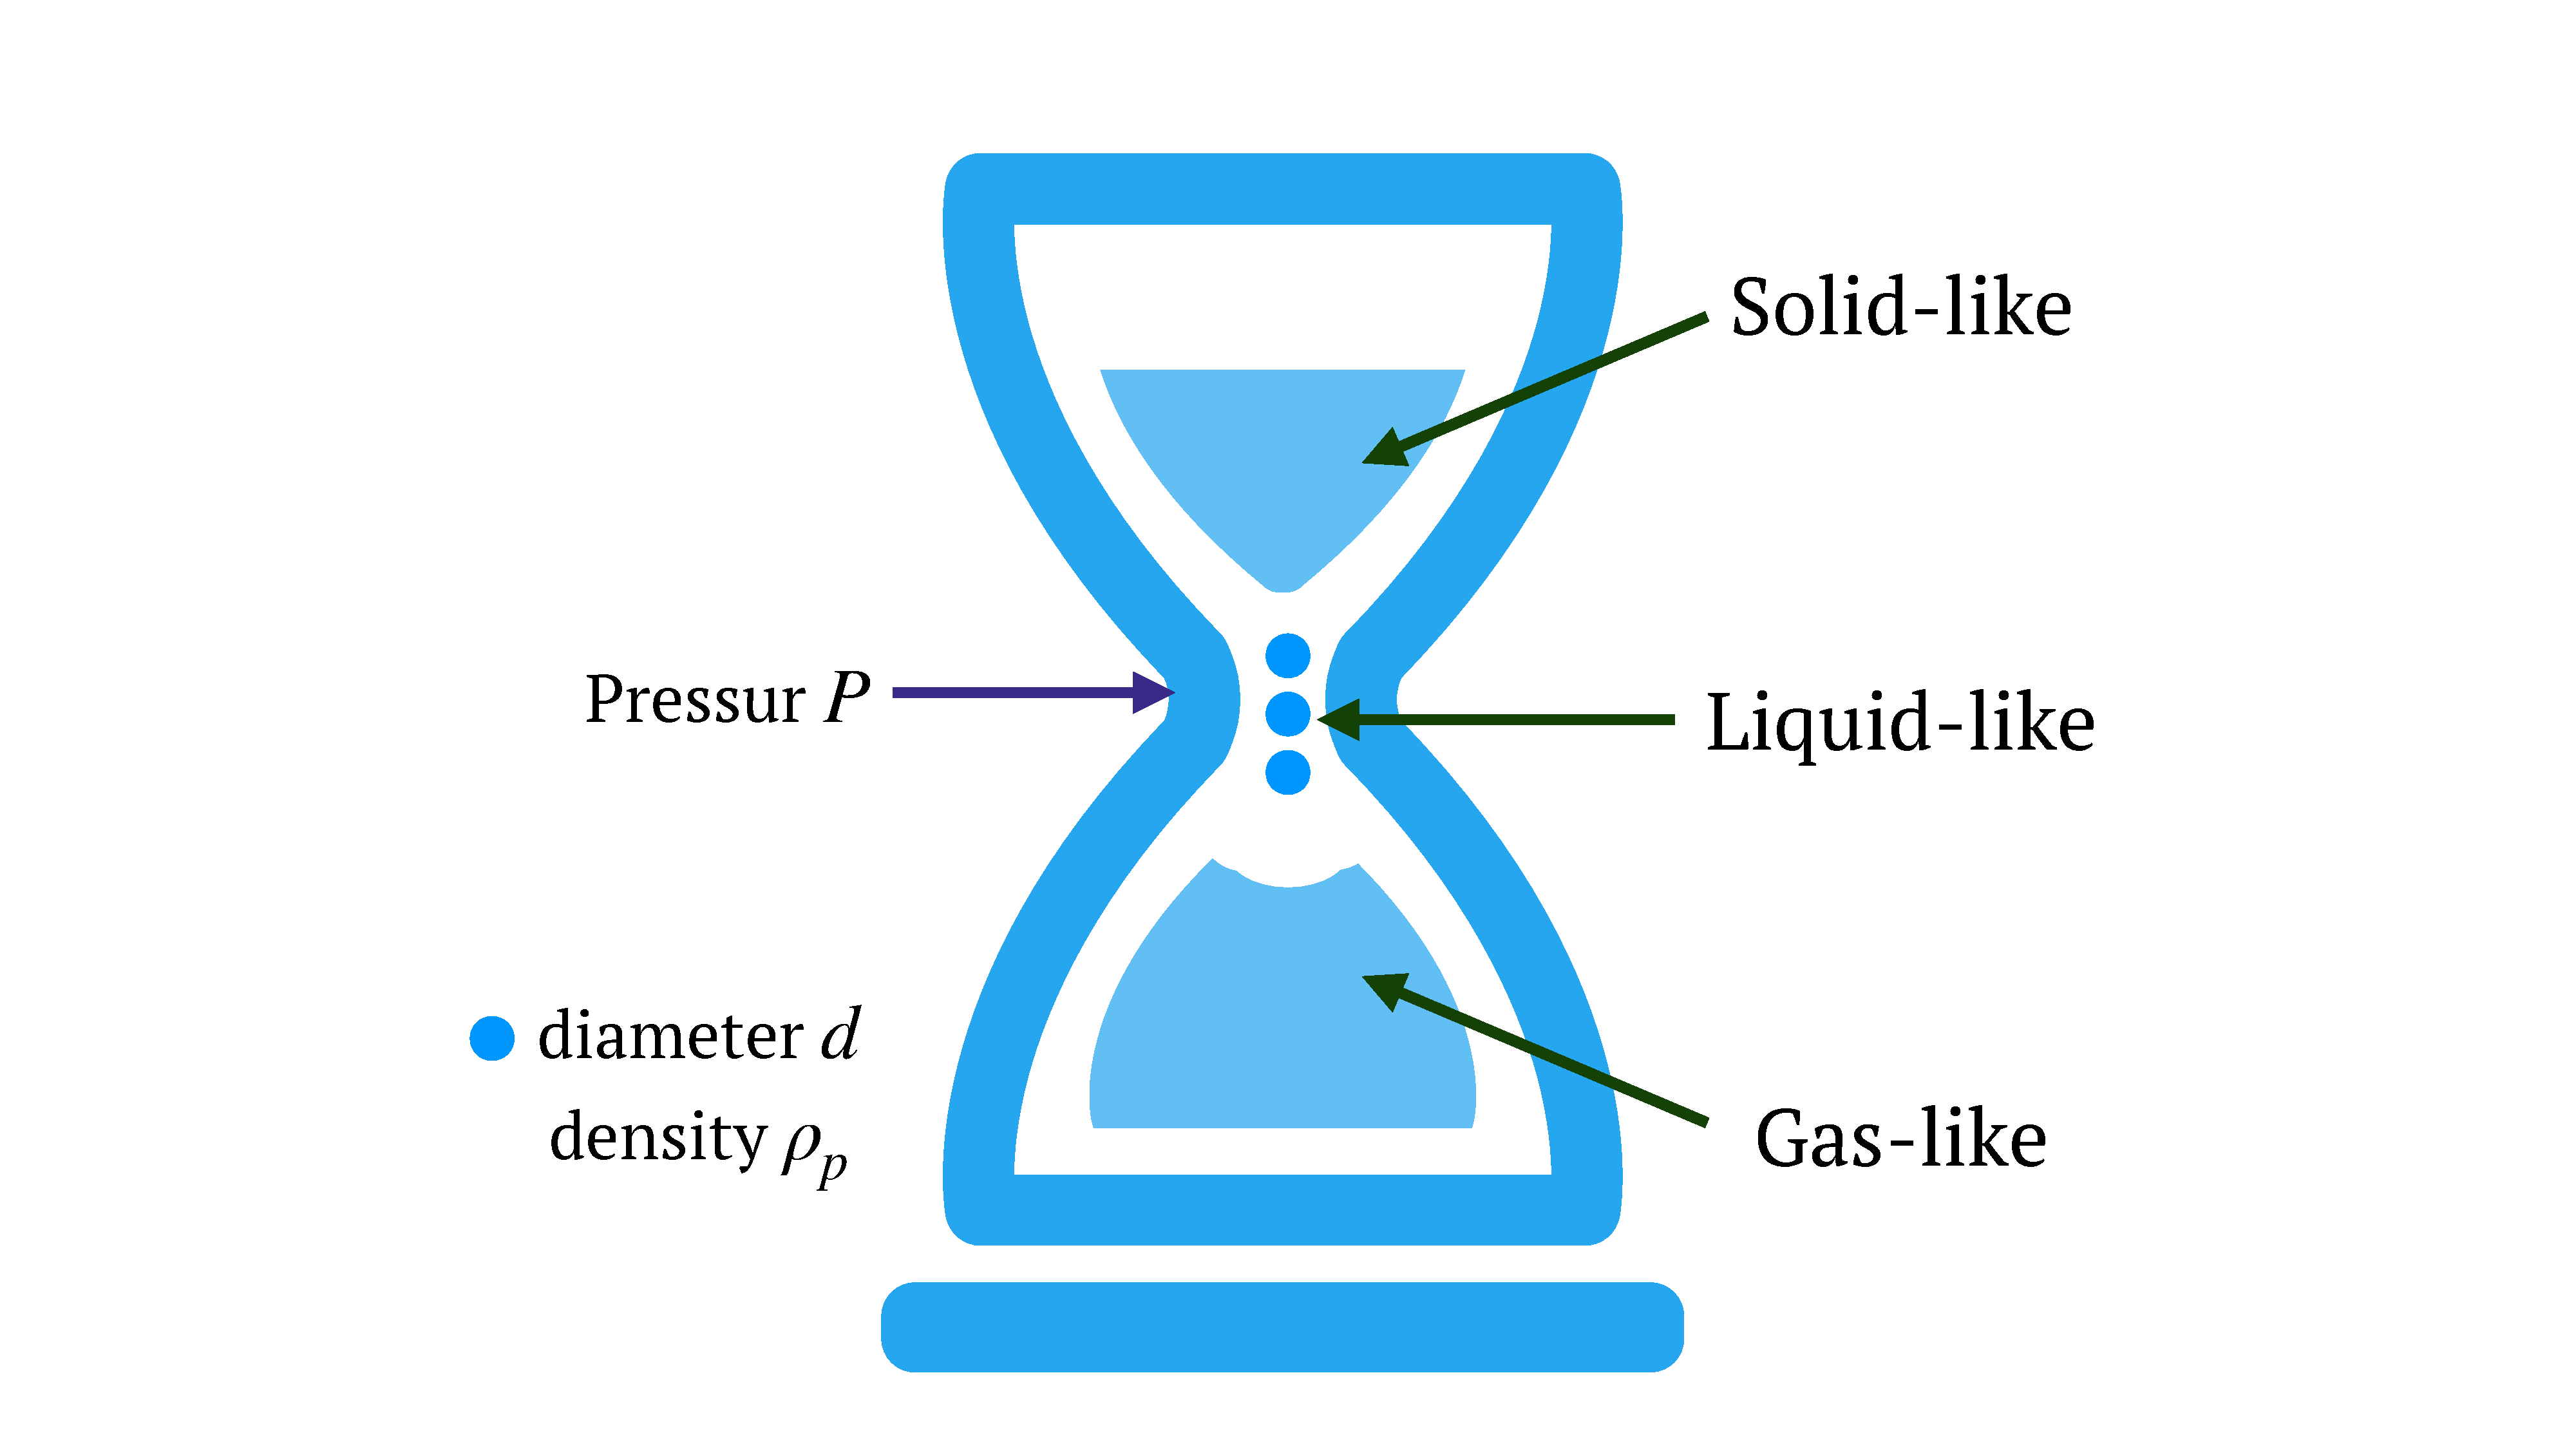
\includegraphics[scale=0.15]{figures/fig_hourglass.pdf}
    \end{center}
  \caption{Schematics of granular flow with an hourglass example.}
  \label{fig_hourglass}
\end{figure}
As we can see in Figure~\ref{fig_hourglass}, three different states can co-exist in granular materials. 
In the top part of the hourglass, filled with sand, the particles seem not to move and resemble a solid. 
In the middle nozzle of the hourglass, we can observe the sands passing through the nozzle, flowing like a liquid.
Meanwhile, the sand landing on the bottom part of the hourglass forms a cone shape. When we look very closely at the top of the cone, we can see that the sand is falling and colliding, behaving like a gas.
\par
In general, these three regimes can be categorized by the inertial number $I$. The solid-like state appears when $I$ is small. As $I$ increases, the granular material deformation occurs rapidly, as we see in the middle of the hourglass. The collisional flow, acting like a gas, can be observed for a large $I$ number. 
\par
By applying this $\mu(I)$ rheology, Srivastava~\cite{srivastava_viscometric_2021} developed a calibration to obtain the coefficients $\eta_i$ and $\kappa_i$, for $i = 1, \ 2$,
\begin{equation}
  \mu_i(I) = \mu_i^0 + A_i{ I}^{ i \alpha_i} =  \frac{(\eta_i \dot{\gamma}^i + \kappa_i)}{P},
\label{eq_muI_general}
\end{equation}
where $\mu_i^0, A_i,$ and $\alpha_i$ are fitting parameters, depending on the materials. 
By substituting the inertial number $I$, equation~(\ref{eq_inertialI}), into equation~(\ref{eq_muI_general}),
we get
\begin{equation}
  \mu_i(I) = \mu_i^0 + A_i {\left(  \frac{\dot{\gamma} d }{\sqrt{P/\rho}}\right) }^{ i \alpha_i} =  \frac{(\eta_i \dot{\gamma}^i + \kappa_i)}{P}.
\label{eq_muI_I}
\end{equation}
We then can find the viscous terms~(\ref{eq_mu1_main}) and~(\ref{eq_mu2_main}),
\begin{equation}
  \mu_i  (\dot{\gamma})= 
 P \Biggl( \mu_i^0 + A_i {\left(  \frac{\dot{\gamma} d }{\sqrt{P/\rho}}\right) }^{ i \alpha_i}\Biggr) 
   \frac{1}{\dot{\gamma}^i}
\label{eq_eta1}
\end{equation}
% For the first-order strain rate viscosity term, equation~(\ref{eq_mu1_main}), we consider the following relationship
% \begin{equation}
%   \mu_1(I) = \mu_1^0 + A_1{ I}^{ \alpha_1} =  \frac{(\eta_1 \dot{\gamma} + \kappa_1)}{P},\
% \label{eq_muI1}
% \end{equation}

% We then find $\mu_1 (\dot{\gamma}, P)$ and $\kappa_1(p)$ as
% \begin{equation}
%   \mu_1  (\dot{\gamma}, P)= 
%   \biggl( A_1 {\left(   d  \sqrt{\rho} \right) }^{ \alpha_1}\biggr) 
%    \dot{\gamma}^{\alpha-1} P^{1-\alpha/2}
% \label{eq_eta1}
% \end{equation}
% \begin{equation}
%     \kappa_1(P) = \mu_1^0 P
% \label{eq_kappa1}
% \end{equation}
% \par
% Similarly, we can find the coefficients for the quadratic in ${\bm D}$ terms, having the $\mu(I)$ relationship as follows:
% \begin{equation}
%     \mu_2(I) = \mu_2^0 + A_2{ I^2}^{ \alpha_1} =  \frac{(\eta_2 \dot{\gamma}^2 + \kappa_2)}{P},\
% \label{eq_muI2}
% \end{equation}
% Then, we obtain $\mu_2 (\dot{\gamma}, P)$ and $\kappa_2(P)$
% \begin{equation}
%     \mu_2  (\dot{\gamma}, P)= 
%     \biggl( A_2 {\left(   d  \sqrt{\rho} \right) }^{ 2\alpha_2}\biggr) 
%      {\dot{\gamma}}^{2(\alpha_2-1)} P^{1-\alpha_2}
% \label{eq_eta2}
% \end{equation}
% \begin{equation}
%     \kappa_2(P) = \mu_2^0 P
% \label{eq_kappa2}
% \end{equation}
%--------------------------------------------------
\noindent
Note that we can obtain the fitting parameters from particle-based simulations for granular materials, such as the discrete element method (DEM). The following parameter values are introduced in~\cite{jop_constitutive_2006} and~\cite{srivastava_viscometric_2021}:
    \[
    0.09 \leq \mu_1^0 \leq 0.33, 
    \ \ \ \ \ \ \ 
    0.37 \leq \alpha_1 \leq 0.7
    \]
        \[
    0.01 \leq \mu_2^0 \leq 0.1, 
    \ \ \ \ \ \ \ 
    0.28 \leq \alpha_2 \leq 0.44.
    \]
One can find the corresponding $A_i$ values in~\cite{srivastava_viscometric_2021}.
Note that we use the following regularization,
\begin{equation}
  \frac{1}{\dot{\gamma}^2} \rightarrow \frac{1-e^{-\dot{\gamma^2} / \varepsilon}}{\dot{\gamma^2}},
\end{equation}
for a higher-order strain rate.
\subsection{Hydrostatic pressure dependency}
For granular rheology, it is typical to see compressible flow. It is, thus, essential to take pressure into account to evaluate the viscosity as seen in equation (\ref{eq_eta1}).
Here, we consider the pressure as a combination of background flow pressure, $P_0$, that is linear in the vertical direction, $z$, and a perturbation, $P'$, such that
\[
P = P_0(z) + P'(x,y,z).\]
Note that the perturbations are due to gravity. Without a gravitational force, we may simply input the pressure, $P_0$, constant over time.
\par
In case gravity is involved, we consider the density term in order to approximate the perturbation, as 
\[
\rho  = \rho_0  + \rho'(x,y,z), 
\]
where $\rho_0$ is constant and $\rho'$ is a spacially-dependent density perturbation of the flow. 
Here, we assume that 
\begin{equation}
    \nabla P_0  = \frac{d P_0}{d z} \approx \rho_0  g.  
\label{eq_p0_rho0}
\end{equation}
This recovers our momentum equation. As we would like to construct a background pressure that stays constant over time for our granular rheology, we may use this assumption.
By integrating both sides of equation~(\ref{eq_p0_rho0}), we obtain
\begin{equation}
    P_0 \approx p_{bg} + \nabla P_0 z.
\end{equation}
We would like to use this form since we already have the $p_{bg}$ term implemented in the AMReX-incflo code.
%
When we have periodic boundary conditions in the gravity direction, we might need to prescribe a pressure gradient to have an additional pressure effect. 
\par
The challenge we faced in implementing the pressure-dependent flow was connecting the pressure in addition to the strain rate into the rheology code. 
We also need to use a different module than the AMReX-incflo for a compressible flow.
% We need to solve for a compressible flow model to have physical consistency using a different numerical solver rather than AMReX-incflo.
We thus leave the pressure-dependent granular flow as a future work.

\section{Numerical method}
In this section, we demonstrate the numerical method used to solve the flow velocity with incompressible Navier-Stokes equations incorporating the viscosity (\ref{eq_eta1}). We particularly focus on the time integration that we wanted to improve as we consider the second-order strain rate stress tensor.
The main AMReX-incflo library provides three different time integration methods: 1) explicit Euler, 2) Crank-Nicolson, and 3) implicit Euler methods. 
Since we have the stress tensor ${\bm \tau}$ of the form~(\ref{eq_CN_tau}), which is non-linear in the velocity, the most convenient choice was the explicit Euler method.
 However, it would be beneficial to have another scheme for more stability, efficiency, and accuracy. 
 \par
 We consider a two-stage Runge-Kutta (RK2) method to achieve second-order convergence. 
In particular, we implemented the following scheme,
\begin{equation}
	\vec{u}^{temp} = \vec{u}^{n} + \frac{\Delta t}{2} {\bm F} \left( \vec{u}^{n} \right)
	\label{eq_RK2_s1} 
\end{equation}
\begin{equation}
	\vec{u}^{*} = \vec{u}^{n} + \Delta t {\bm F} \left( \vec{u}^{temp} \right),
	\label{eq_RK2_s2}
\end{equation}
where 
\[
  {\bm F} \left( \vec{u}^{n} \right)= 
    -\vec{u}^n \cdot \nabla \vec{u}^n 
    +\frac{1}{\rho}
    \biggl(
    - \nabla P^n 
        + \nabla \cdot   \bm{\tau}(\vec{u}^n)
        +  \rho  \vec{g} 
        \biggr).
\]
where the superscript $n$ represents the current time (known) value; $\vec{u}^n \approx \vec{u}(\vec{x}, t_n)$. The new velocity value $\vec{u}^*$ is an updated velocity to the next time, $\vec{u}^*  \approx \vec{u} (\vec{x}, t_{n+1})$. 
Note that the \textit{temp} time is considered to be $ n + n$/2. One important part of being consistent is that we only update the one time step with $\Delta t$, from the time $n$ to $*$. 
\par
After we integrate over one time step, we should make sure that $\vec{u}^*$ satisfies the continuity equation~(\ref{eq_conserv_mass}). We thus project this intermediate velocity $\vec{u}^*$ onto the divergence-free space~\cite{sverdrup_highly_2018}.
For the projection step, we first express $\vec{u}^{*}$ according to the Helmholtz-Hodge-Decomposition~\cite{chorin_mathematical_1993}, 
\begin{equation}
  \vec{u}^* = \vec{u}^{n+1} + \nabla \phi,
  \label{eq_ustar}
\end{equation}
where $\vec{u}^{n+1}$ is the new velocity at time $t_{n+1}$ that satisfies the divergence-free condition and $\phi$ is a scalar function.
To take advantage of the incompressibility of $\vec{u}^{n+1}$, we find the divergence of equation~(\ref{eq_ustar}), leading to the Poisson equation for $\phi$,
\[
  \nabla^2 \phi = \nabla \vec{u}^*.  
\]
After we solve for $\phi$, applying given boundary conditions, we find the updated velocity, projecting the velocity $\vec{u}^*$ onto the divergence-free space to get the new time-level solutions.
\[
  \vec{u}^{n+1} = \vec{u}^* - \nabla \phi.
\]
As we mentioned, my contribution to the AMReX-incflo for this project is the granular material viscosity evaluation and the RK2 scheme implementation. For the rest of the parts to solve for the Navier-Stokes equations, we use the AMReX-incflo library as it is. Note that the details of general algorithms for this library can be found in~\cite{almgren_conservative_1998}.
% In the following section, we validate the implementation of the RK2 scheme with second-order granular rheology. We should mention that the order convergence might not be recovered due to the higher-order tensor computations and projection step. Nonetheless, we expect to obtain a better convergence rate and better accuracy with the RK2 method compared to explicit Euler.

% {\color{blue} Are we keeping this the whole time? Is there any pressure change over time? Does a volume fraction come into play?}

% a little more details
%---subsection---what I did not do-------
\begin{comment}
\subsection{Predictor-Corrector method}
To enlarge the numerical stability region, we implement a semi-implicit method. To do so, we first re-write the momentum equation by splitting the deviatoric stress tensor, ${\bm \tau}$, into two parts, 
\[
 {\bm \tau}= {\bm \tau_1} + {\bm \tau_2},
\] 
where ${\bm \tau_1}$ and ${\bm \tau_2}$ are, respectively, the linear and quadratic relationship with ${\bm D}$, i.e., 
\[
  {\boldsymbol \tau_1} \propto \boldsymbol{D}
  \ \ \ \ \ \text{and}
   \ \ \ \ \ 
{\boldsymbol \tau_2} \propto {\boldsymbol D^2}.
\]
We denote the advection term, $\vec{u} \cdot \nabla \vec{u}$ as ${\bm A}$. 
\\
$<${\bf Predictor}$>$
\\
First, consider the non-linear stress tensor, ${\bm \tau_2}$ as a force term, and solve for the first predictor values, that are $\vec{u}^*$ and $\vec{u}^*$:
\[
\frac{{\color{blue}\vec{u}^*} - \vec{u}^n}{\Delta t} 
+  {\bm A}^{n+1/2} 
= \frac{1}{\rho}  \biggl(
\frac{\nabla \cdot {\color{blue}{\bm \tau}_1^*} + \nabla \cdot{\bm \tau}_1^n}{2} 
+ \nabla \cdot {\bm \tau}_2^n 
- \nabla p^n
+{\bm g}
\biggr)
\]
We solve for blue terms - 
\[
{\color{blue}\vec{u}^*} -
\frac{\Delta t}{\rho} 
\left( 
\frac{\nabla \cdot {\color{blue}{\bm \tau}_1^*}}{2}
\right)
=
\vec{u}^n
- {\bm A}^{n+1/2} \Delta t
+ \frac{\Delta t}{\rho} \biggl(
\frac{ \nabla \cdot{\bm \tau}_1^n}{2} 
+ \nabla \cdot {\bm \tau}_2^n 
- \nabla p^n
+{\bm g}
\biggr)
\]
\\
$<${\bf Corrector}$>$
\\
Once we obtain the predictor (star) velocity, we use it to compute the second order stress tensor, ${\bm \tau}_2^*$.
\[
\frac{{\color{red}\vec{u}^{n+1}} - \vec{u}^n}{\Delta t} 
+  {\bm A}^{n+1/2} 
=  \frac{1}{\rho}  \biggl(
\frac{\nabla \cdot {\color{red}{\bm \tau}_1^{n+1}} + \nabla \cdot{\bm \tau}_1^n}{2} 
+ \frac{\nabla \cdot {\bm \tau}_2^{n} + \nabla \cdot {\color{blue}{\bm \tau}_2^*}}{2} 
- \nabla p^n
\biggr)
\]

Now, we need to solve for red - next time step values:
\[
{\color{red}\vec{u}^{n+1}} 
-\frac{1}{\rho} 
\left(
\frac{\nabla \cdot {\color{red}{\bm \tau}_1^{n+1}}}{2}
\right)
=
\vec{u}^n 
 -{\bm A}^{n+1/2} \Delta t
 +\frac{\Delta t}{\rho}  \biggl(
\frac{ \nabla \cdot{\bm \tau}_1^n}{2} 
+ \frac{\nabla \cdot {\bm \tau}_2^{n} + \nabla \cdot {\color{blue}{\bm \tau}_2^*}}{2} 
- \nabla p^n
\biggr)
\]
Note that ${\bm \tau}_i^* = {\bm \tau}(\vec{u}^*, \eta_i)$.
\end{comment}
\section{Numerical validation for time integration}
We compare the performance of time integration methods: 1) the explicit Euler, which was already available in the AMReX-incflo, and 2) the explicit RK2 scheme that we implemented for a higher-order strain rate rheology.
\begin{figure}[ht]
  \begin{center}
    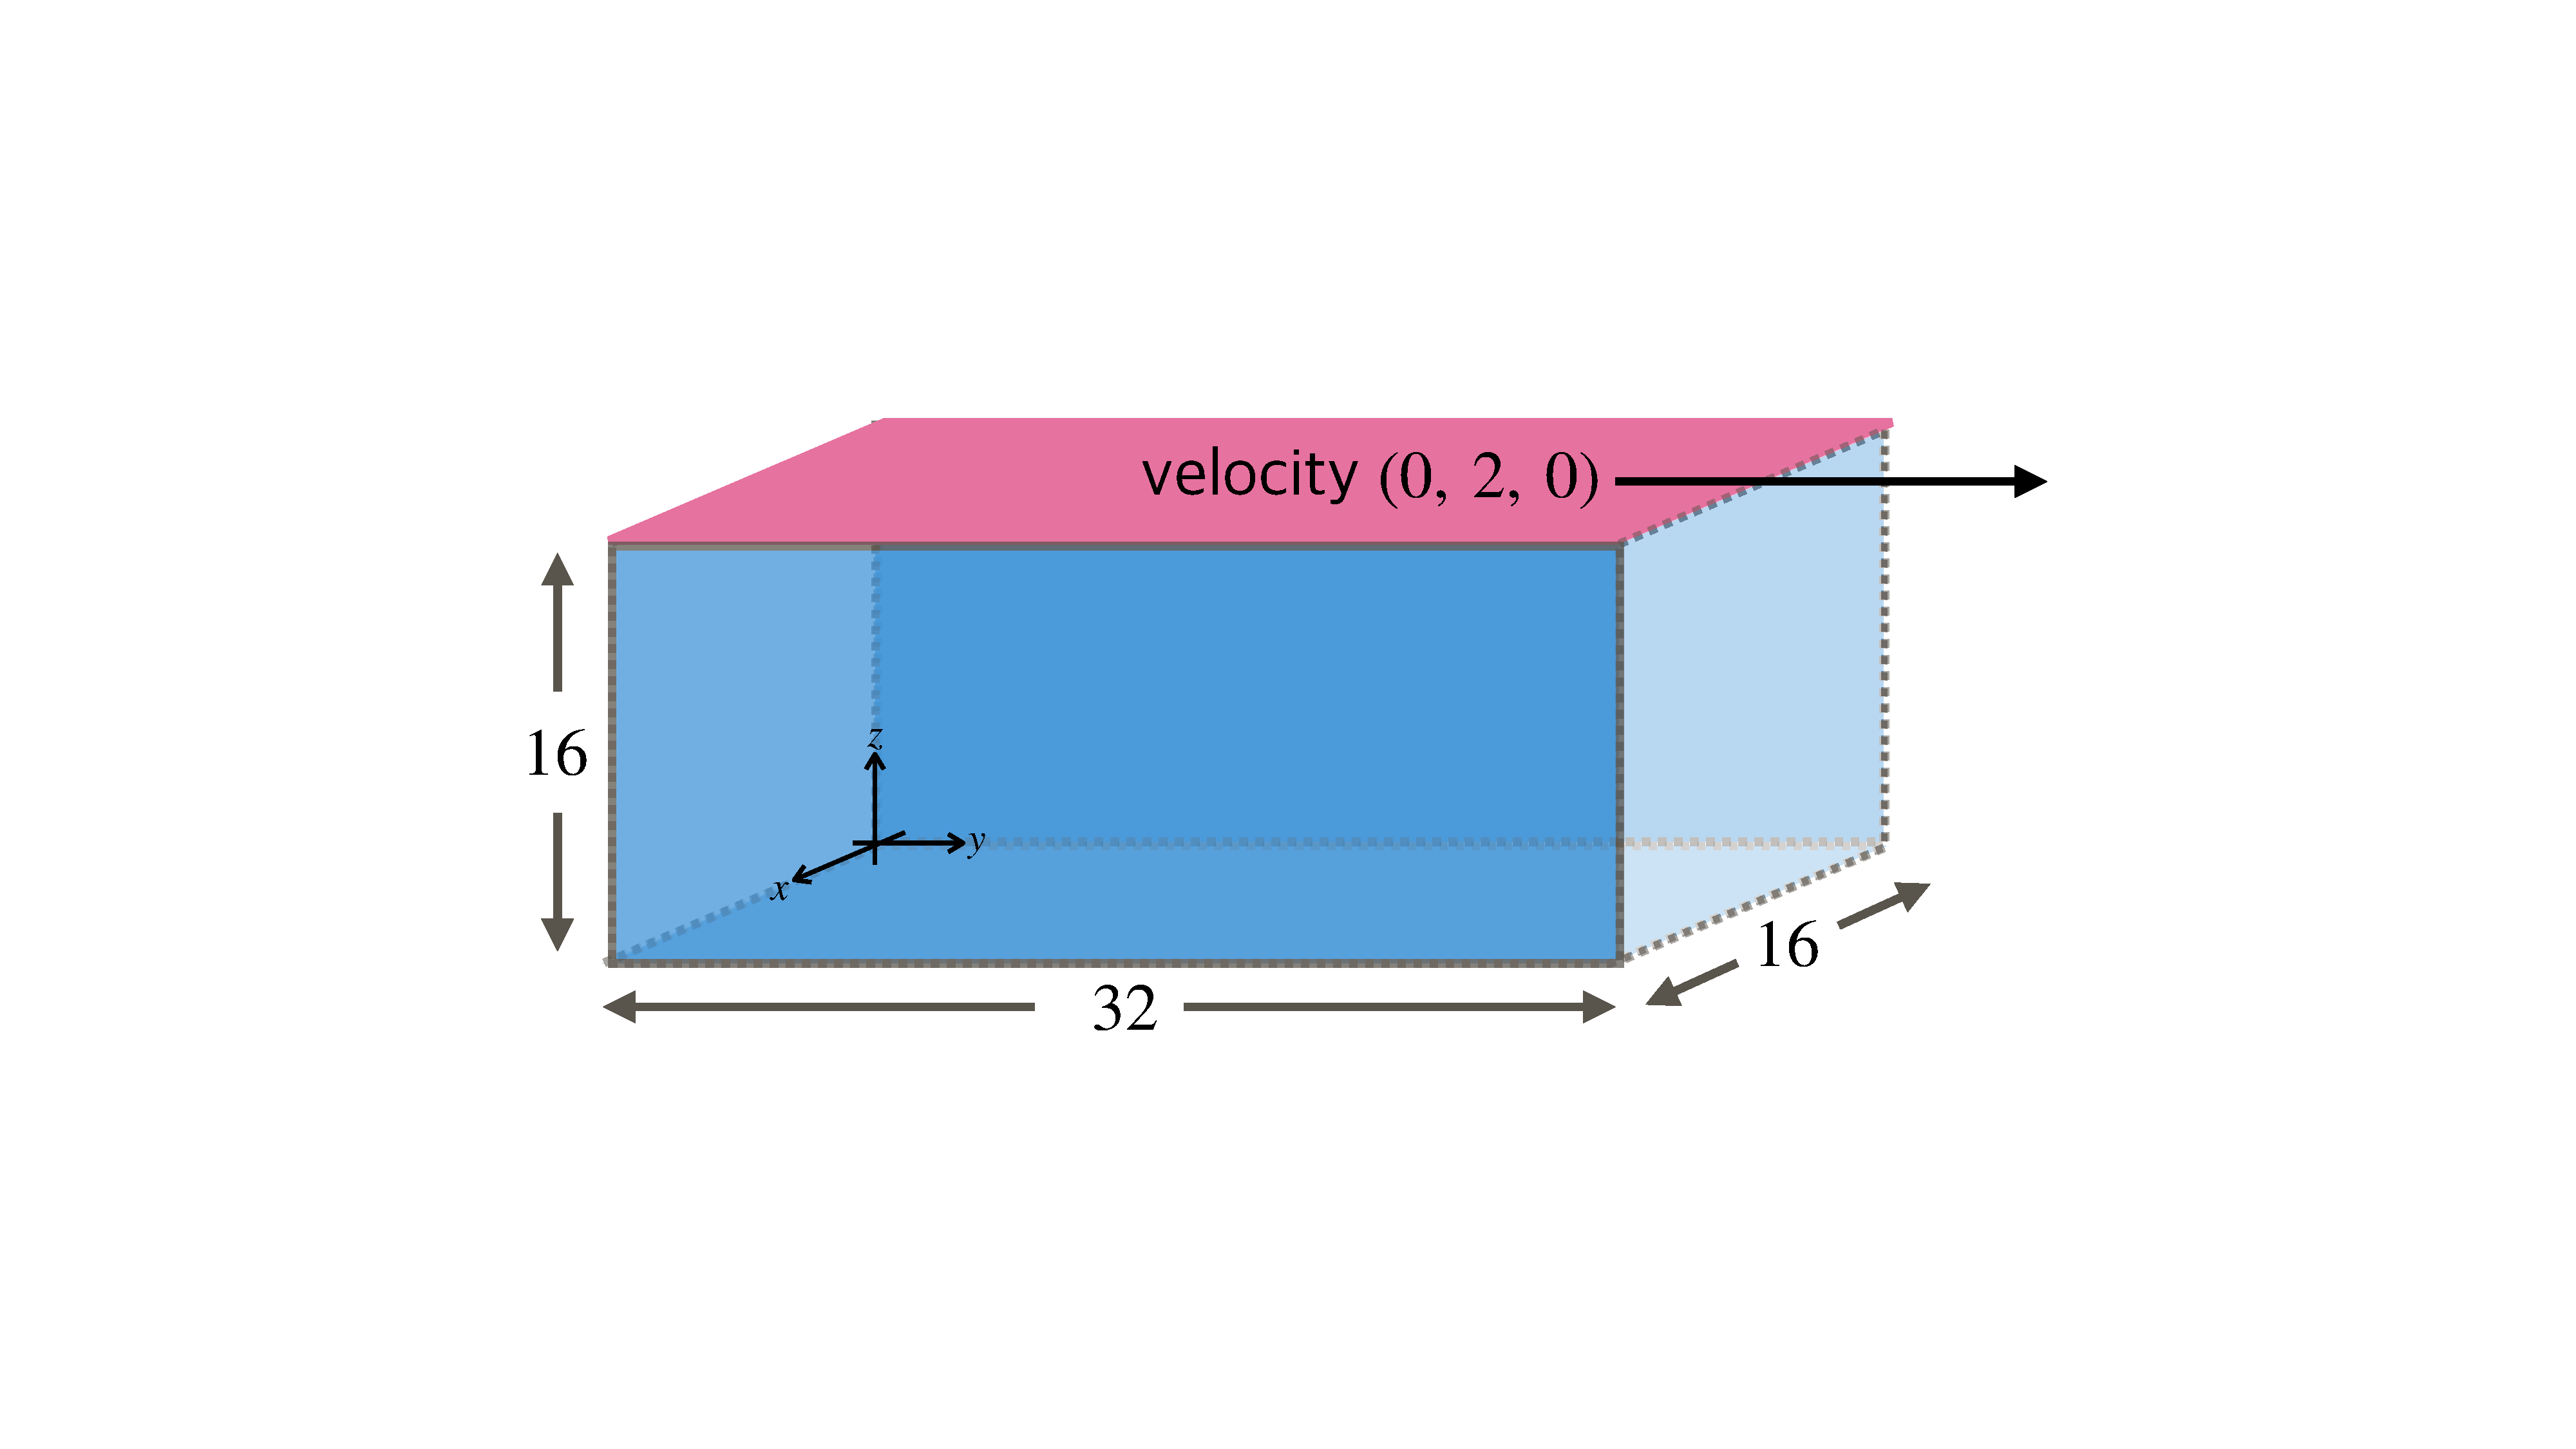
\includegraphics[scale=0.3]{figures/fig_granular_domain.pdf}
    \end{center}
  \caption{Numerical simulation domain box filled with sand type material. We use dimensions with centimeters for a length and seconds for a time scale.}
  \label{fig_granular_domain}
\end{figure}
\par
For this validation, we consider a rectangular cuboid, as we show in Figure~\ref{fig_granular_domain}, with dimensions $2 \text{ cm} \ (x) \times 1 \text{ cm} \  (y) \times 2 \text{ cm} \ (z)$, where all the walls in the $x-$ and $z-$directions have a no-slip boundary condition. We impose a periodic condition on the $y-$direction. Note that we consider centimeters (cm) for the length scale. 
In the finite volume sense of spatial discretization, the total number of cells composing the cuboid is $8 \times 8 \times 8$.
% the number of cells composed of the cuboid is the same as the dimensions of the cuboid, i.e., each cell size is $1 \times 1 \times 1$. 
We suppose this cuboid is filled with dry sands of a mean diameter $d = 0.15$ cm and material density $\rho = 1$ g/cm$^3$. To make sands flow, we move the top plate in the $y-$direction, shown as the pink in Figure~\ref{fig_granular_domain}, with the velocity (0, 1, 0) cm/s.
For the rest of the parameters, we obtain information from other research papers.
In~\cite{senetakis_inter-particle_2013}, they observed the interparticle friction of dry sands $\mu_s \approx 0.01$~g$\cdot$cm/s$^2$, in which particle sizes are in the range of 0.12 cm and 0.24 cm. 
% of~$0.12\text{ cm} \leq d \leq 0.24$~cm. 
We then find the fitting parameters from~\cite{srivastava_viscometric_2021}, as in the following Table~\ref{table_test}. 
\begin{table}[ht]
  \resizebox{\textwidth}{!}{%
   \begin{tabular}[ht]{|c|c|c|c|}
   \hline
   & \hspace{1.5cm} $\mu_i^0$ \hspace{1.5cm} & \hspace{1.5cm} $\alpha_i$ \hspace{1.5cm} &   \hspace{1.5cm}$A_i$   \hspace{1.5cm} \\  \hline
   \hspace{1cm} $i = 1$ \hspace{1cm}   & \hspace{1.5cm} 0.12 \hspace{1.5cm} & \hspace{1.5cm} 0.41 \hspace{1.5cm} & \hspace{1.5cm}  0.512 \hspace{1.5cm}
       \\  \hline
       \hspace{1cm} $i = 2$ \hspace{1cm} & \hspace{1.5cm}  0.02 \hspace{1.5cm} & \hspace{1.5cm} 0.31 \hspace{1.5cm} & \hspace{1.5cm} 0.252 \hspace{1.5cm}
  \\ 
  \hline
  \end{tabular}}
\caption{Fitting parameters of granular materials when the interparticle friction~$\mu_s = 0.01$~\cite{srivastava_viscometric_2021}.
}
\label{table_test}
\end{table}
With this setup and parameters, we first observe the finest results to understand the flow.  
\subsection{Velocity in the shear flow direction}
 We first present the reference solution of our simulation. In particular, we show the velocity in the shear flow direction, $y$, in Figure~\ref{fig_reference_3d_T110}.
\begin{figure}[ht]
\begin{center}
  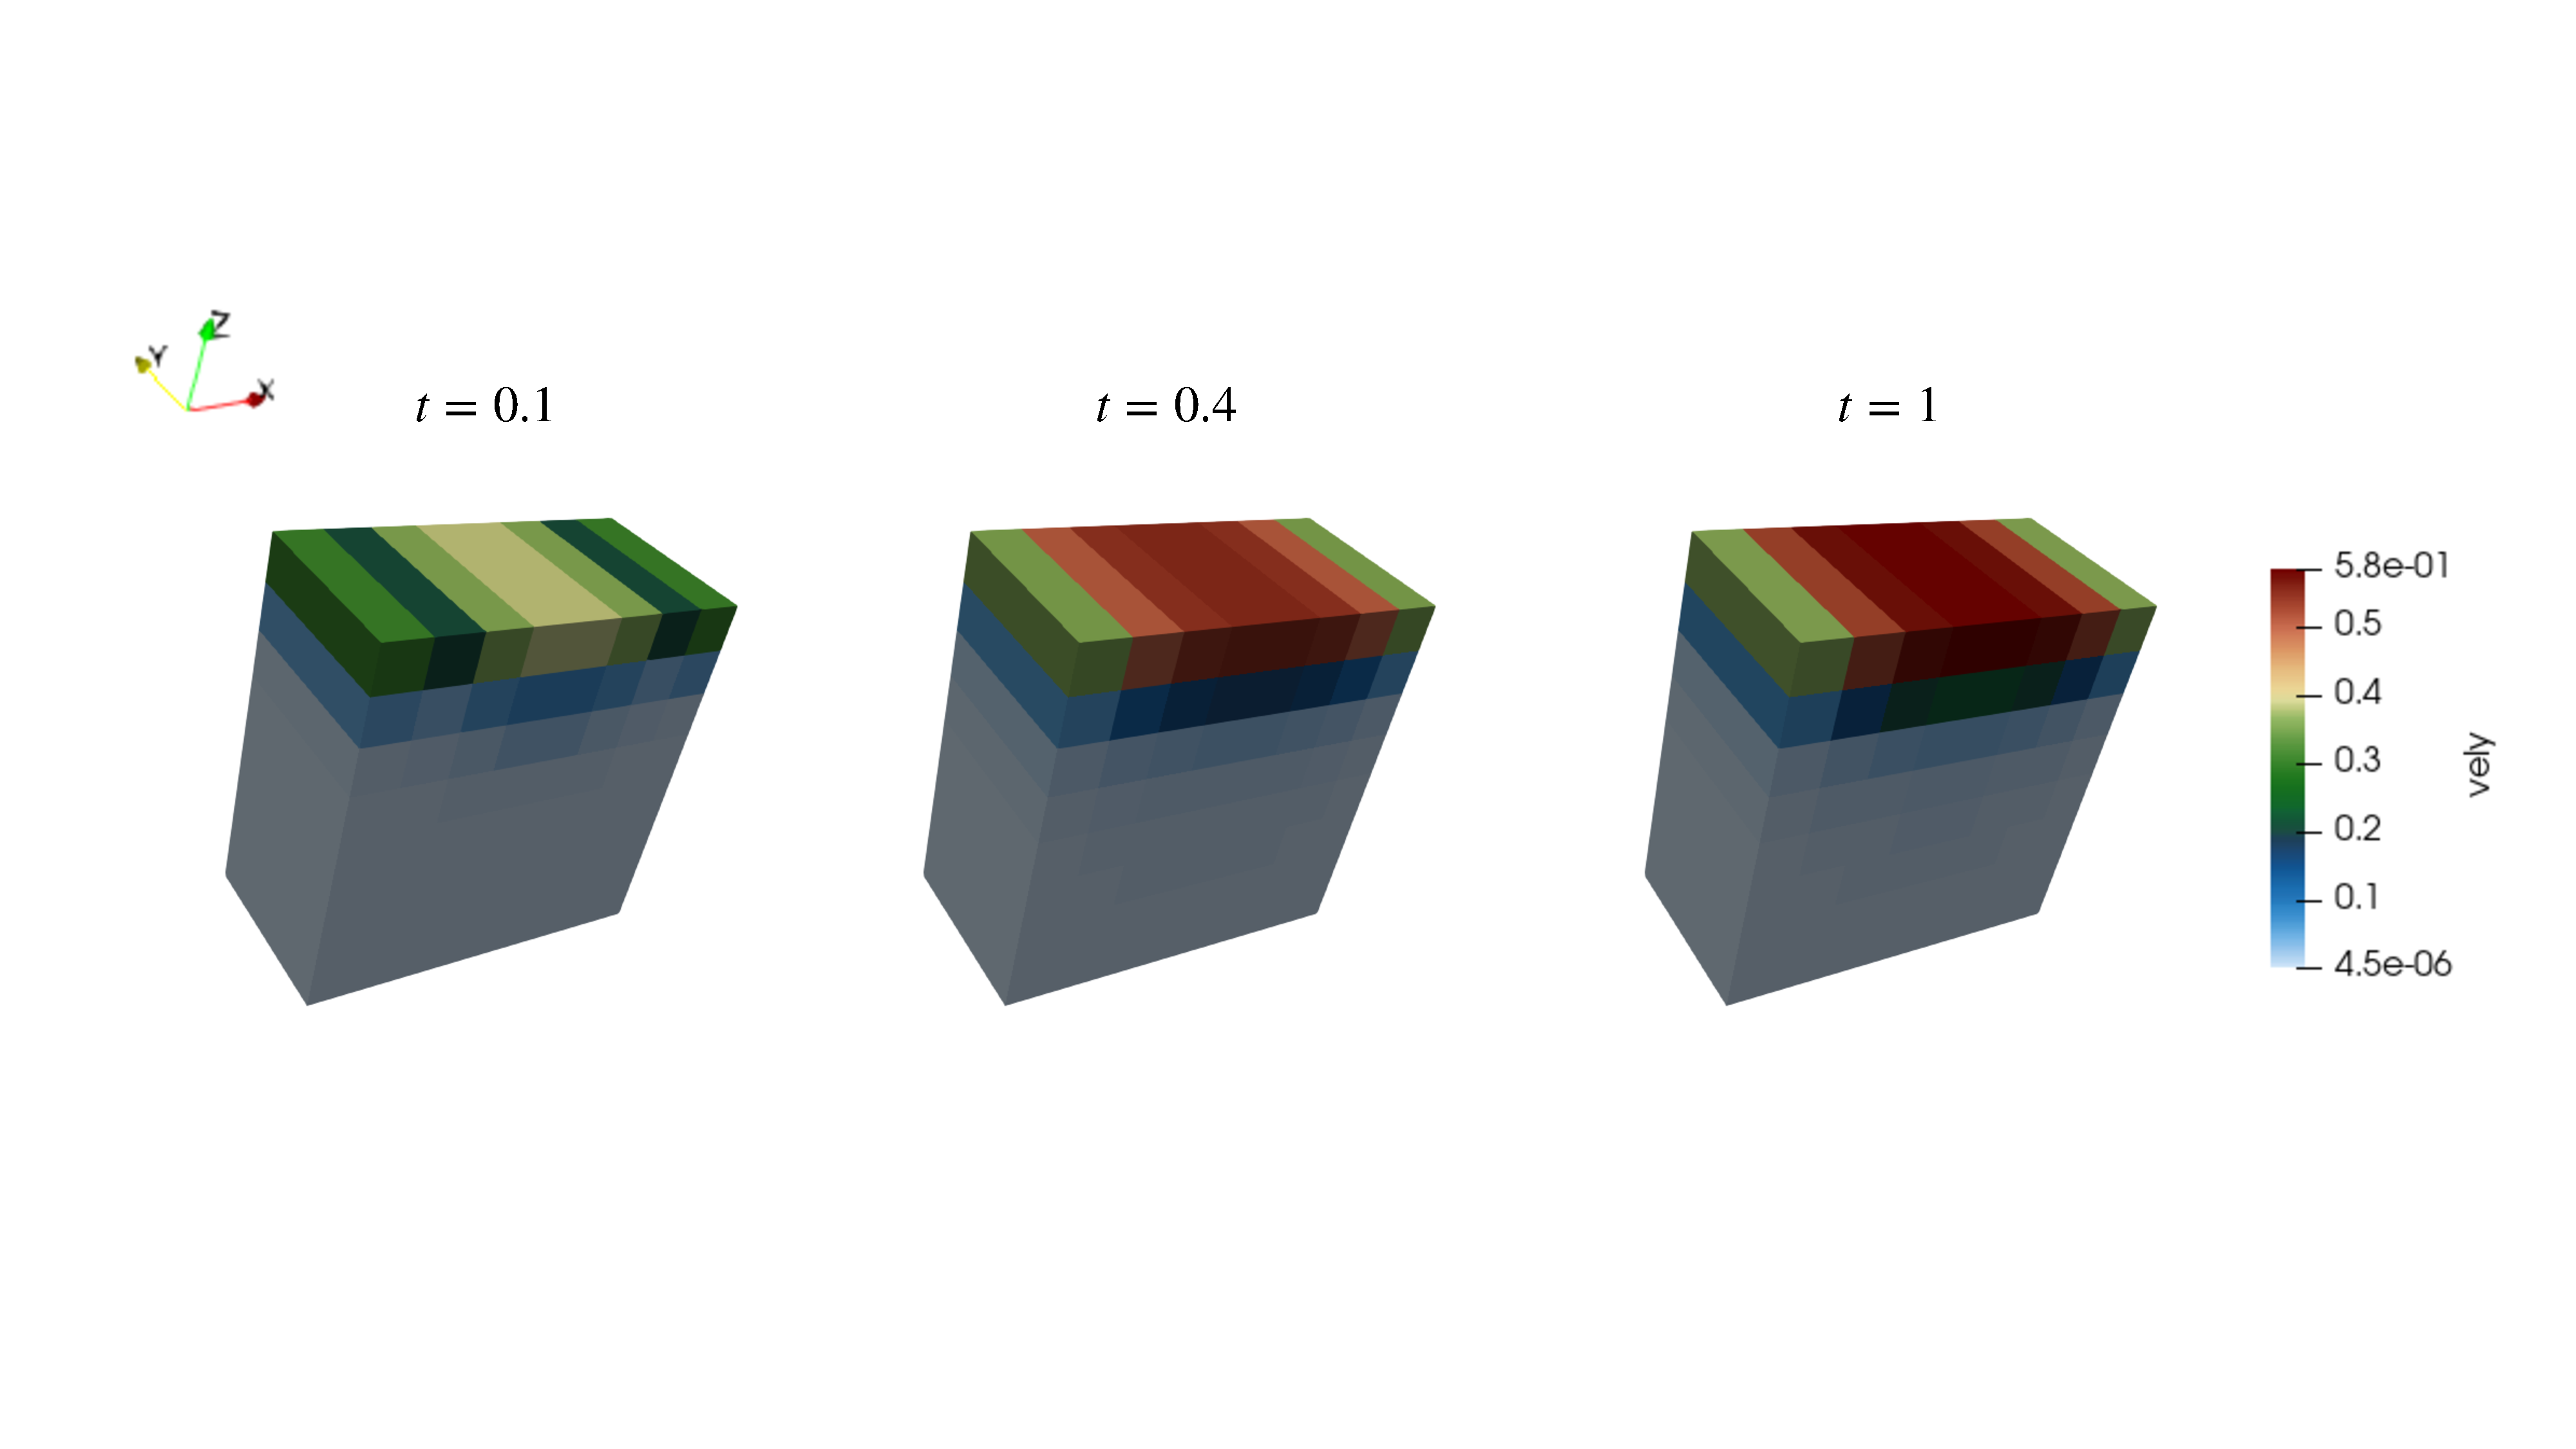
\includegraphics[scale=0.23]{figures/fig_reference_3d_T110.pdf}
  \end{center}
\caption{Velocity component (cm/s) in $y-$axis at time $t = 0.1, \ 0.4$ and $t = 1$ (s).}
\label{fig_reference_3d_T110}
\end{figure}
We use the explicit Euler method with the time step $\Delta t = 10^{-5}$ (s) as the reference solution. The final time of this validation is $t = 1$ s.
\begin{figure}[ht]
  \begin{center}
    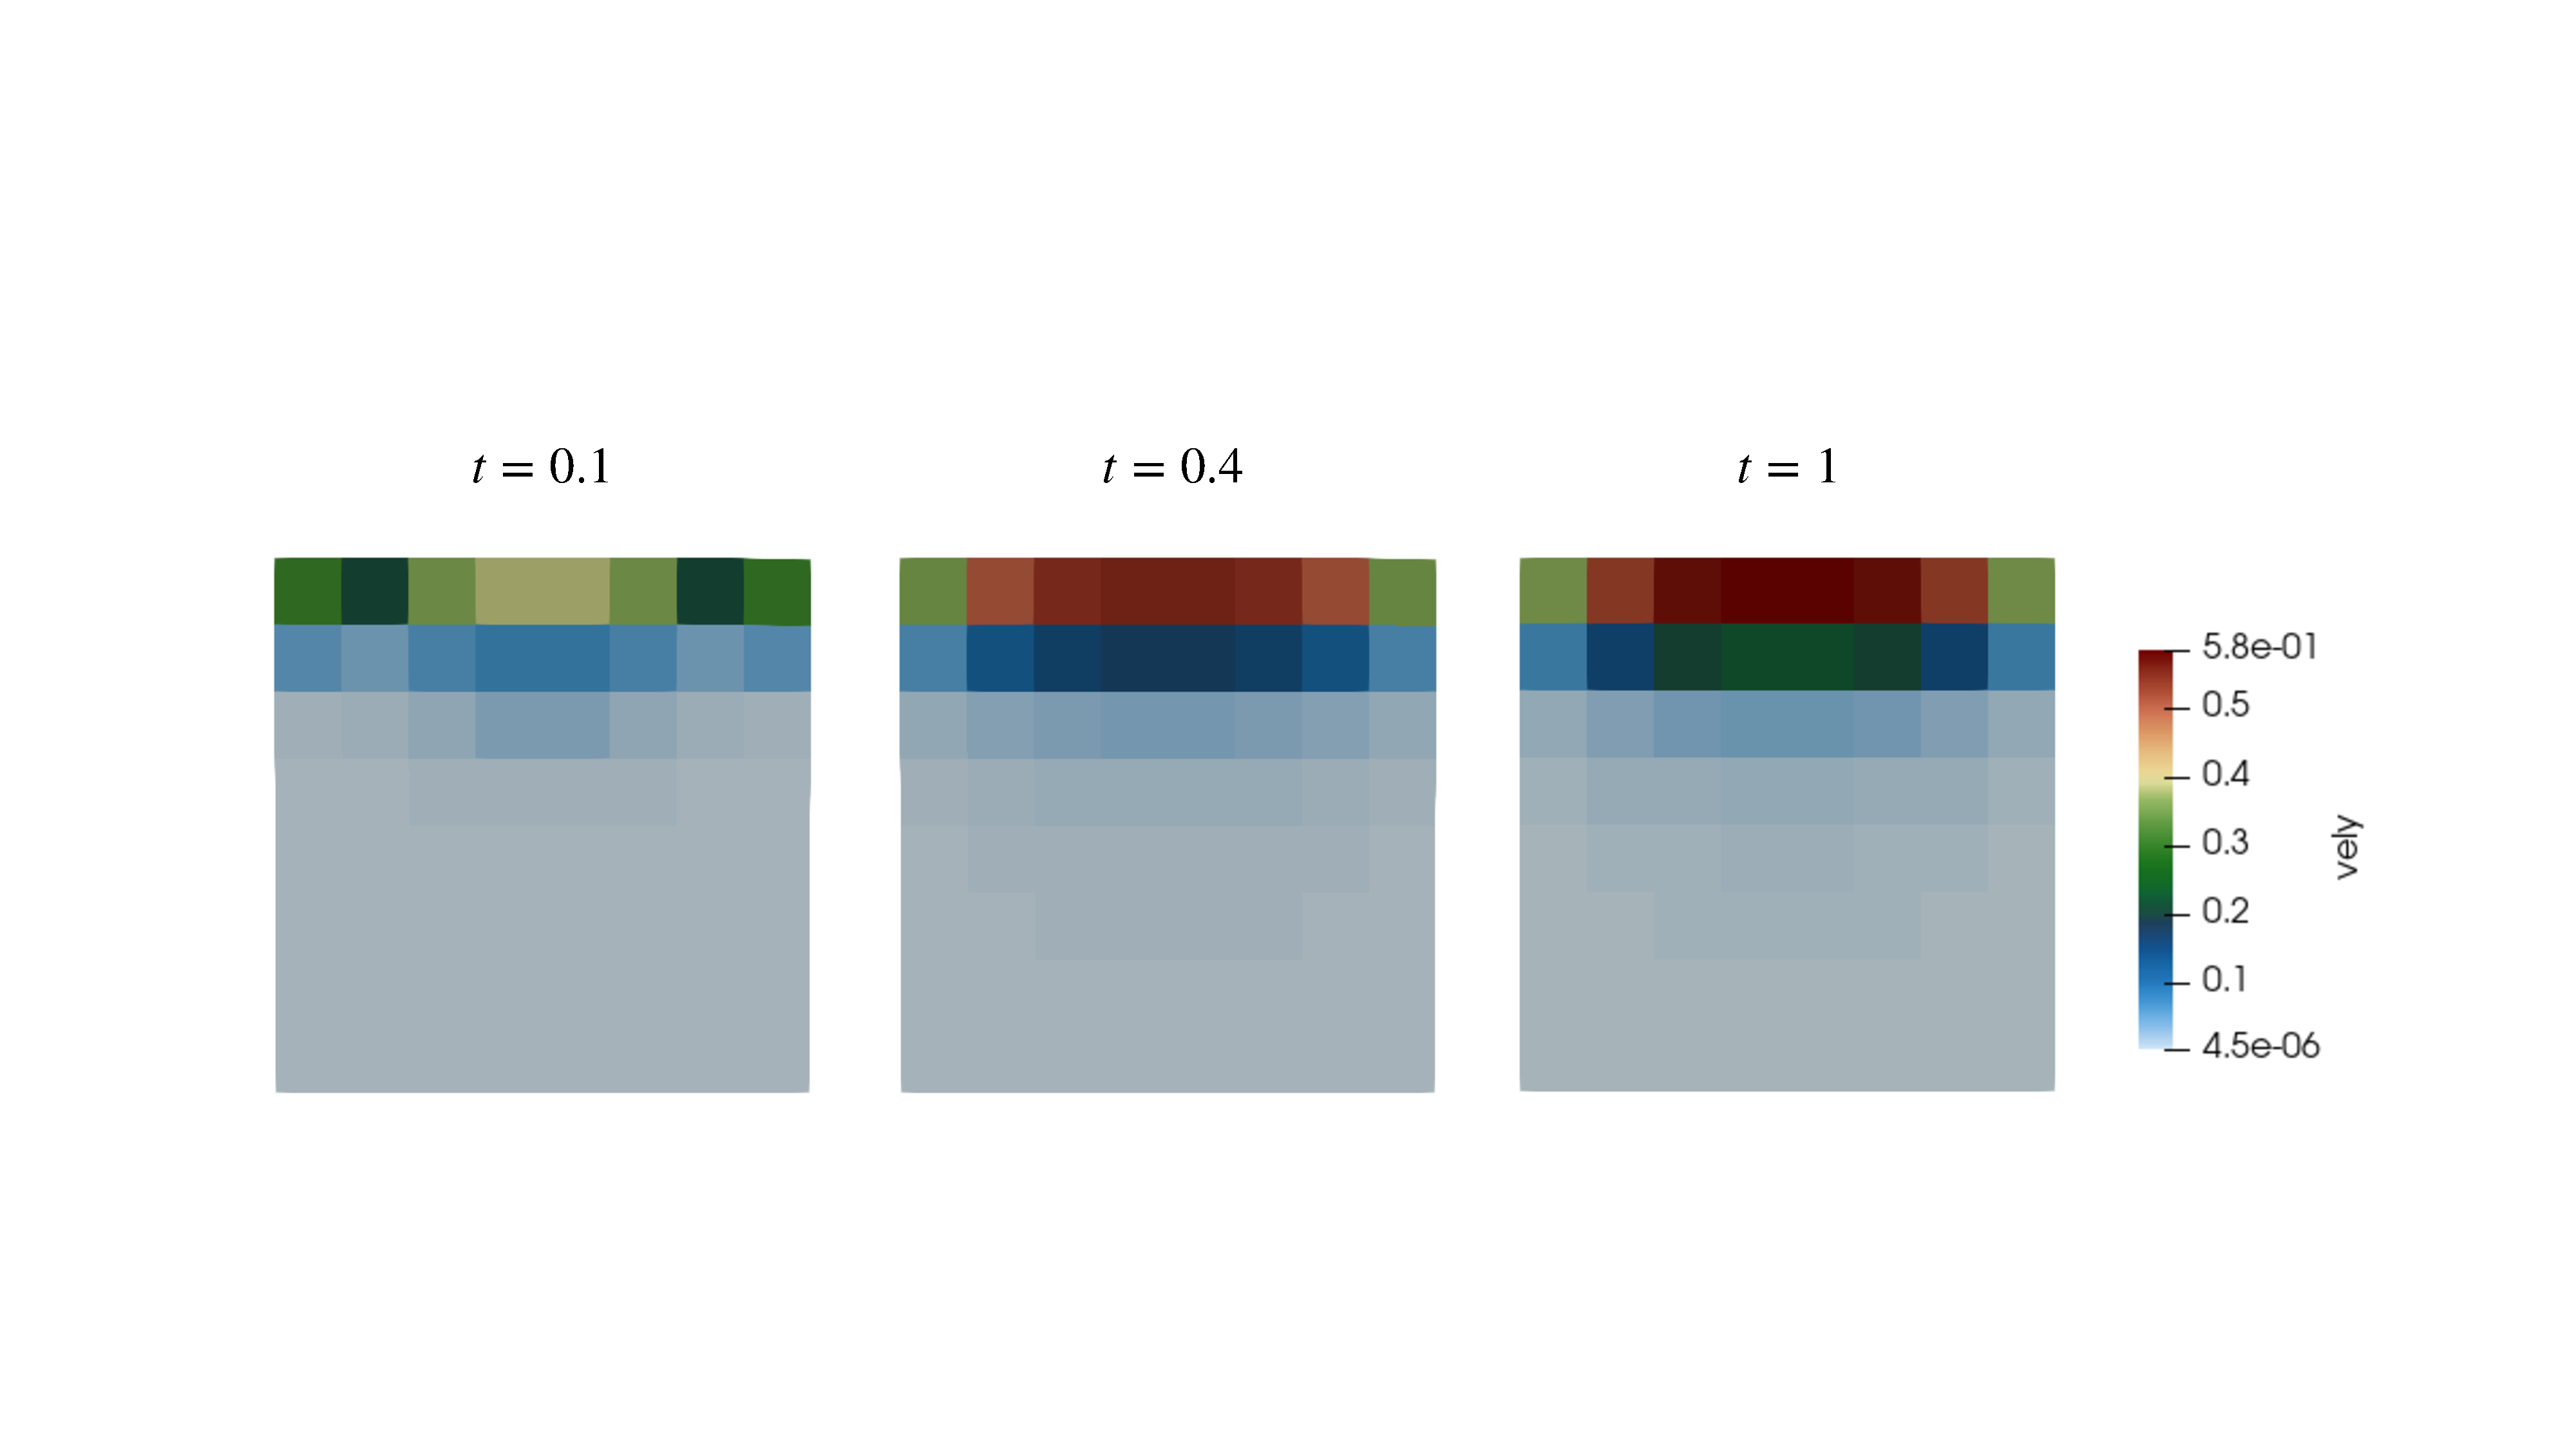
\includegraphics[scale=0.25]{figures/fig_reference_T1610.pdf}
    \end{center}
  \caption{Velocity component (cm/s) in $y-$axis at time $t = 1, 6,$ and 10 (s).}
  \label{fig_rerference_T1}
\end{figure}
\par
We note that in this setup, the velocity is independent of $y$, although we move the plate in this direction. To observe the variation of $x-z$ plane clearly, we obtain Figure~\ref{fig_rerference_T1} when $y = 1$. We can see that the most variation occurs on the top of the $z$-axis where the plate is moving. 

\subsection{Error analysis (order convergence)}
Using the reference velocity in $y-$direction obtained by the explicit Euler, we get the errors of the Euler and RK2 methods with various time step sizes, $\Delta t$. 
In Figure~\ref{fig_second_order_compare_err_time}, we obtain the infinite norm of the absolute difference of velocities in the $y-$axis. 
It is clear to see that RK2 is performing much better in terms of order convergence and accuracy. 
\begin{figure}[h]
  \begin{center}
    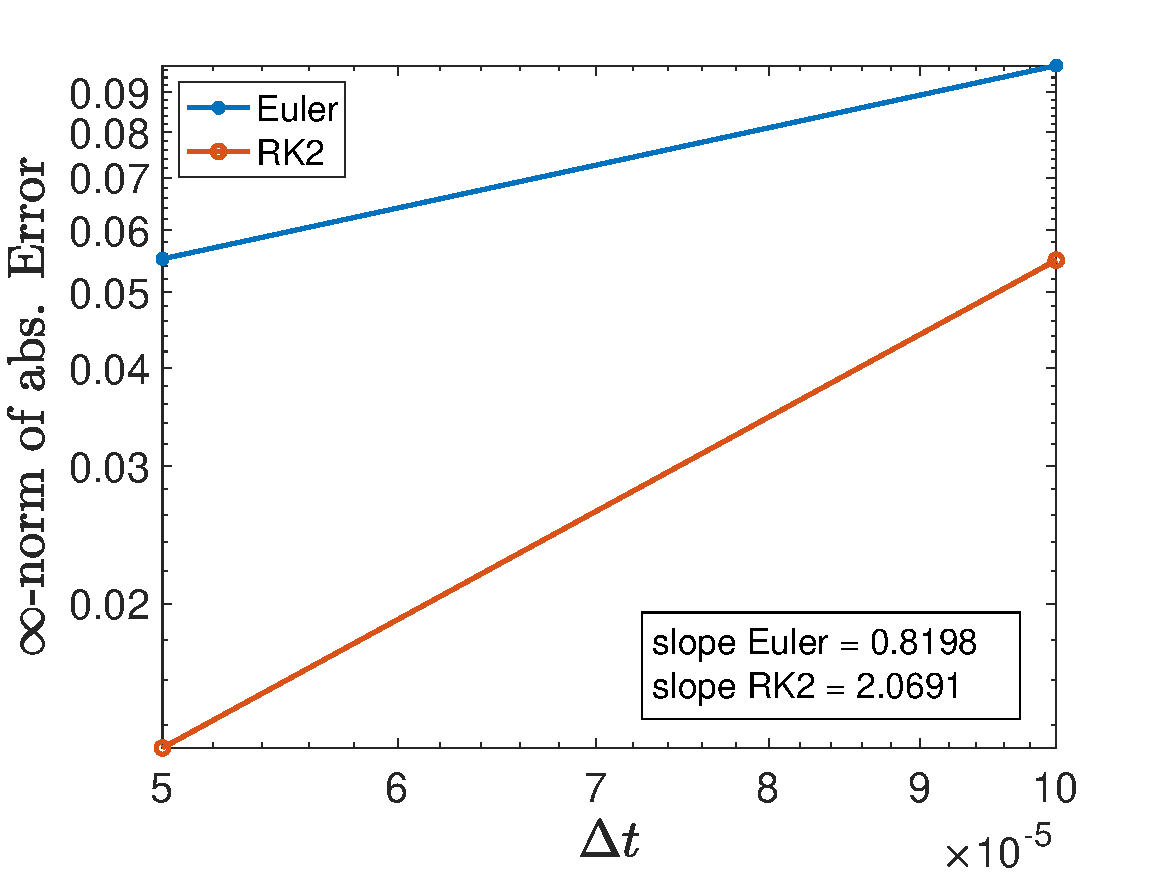
\includegraphics[scale=0.4]{figures/fig_granular_box212_8cube_infnorm}
    \end{center}
  \caption{Order convergence between the explicit Euler and RK2 schemes at time $t = 1$ (s). The vertical axis shows the infinite norm of the absolute differences between the reference solution and each method.}
  \label{fig_second_order_compare_err_time}
\end{figure}
\par
As we expected, the explicit Euler method shows close to the first order, and the RK2 shows second-order convergence. Note that due to the time constraint, we used two points, $\Delta t = 10^{-4}, \ 50^{-5}$, to plot Figure~\ref{fig_second_order_compare_err_time}. Since the error of the explicit Euler method is large and we need the Euler method for a reference solution to validate the RK2 scheme, we have to use quite a small time step $\Delta t$ to confirm the convergence. 
\section{Future work}
There are several potential future works we could consider as an extension of this project. 
We may analyze the stabilities between the explicit Euler and RK2 methods for this particular granular flow in the cuboid.
Our preliminary results of the new time integral implementation showed that the RK2 method was more stable than the explicit Euler method for certain fitting parameters.
\begin{figure}[ht]
  \begin{center}
    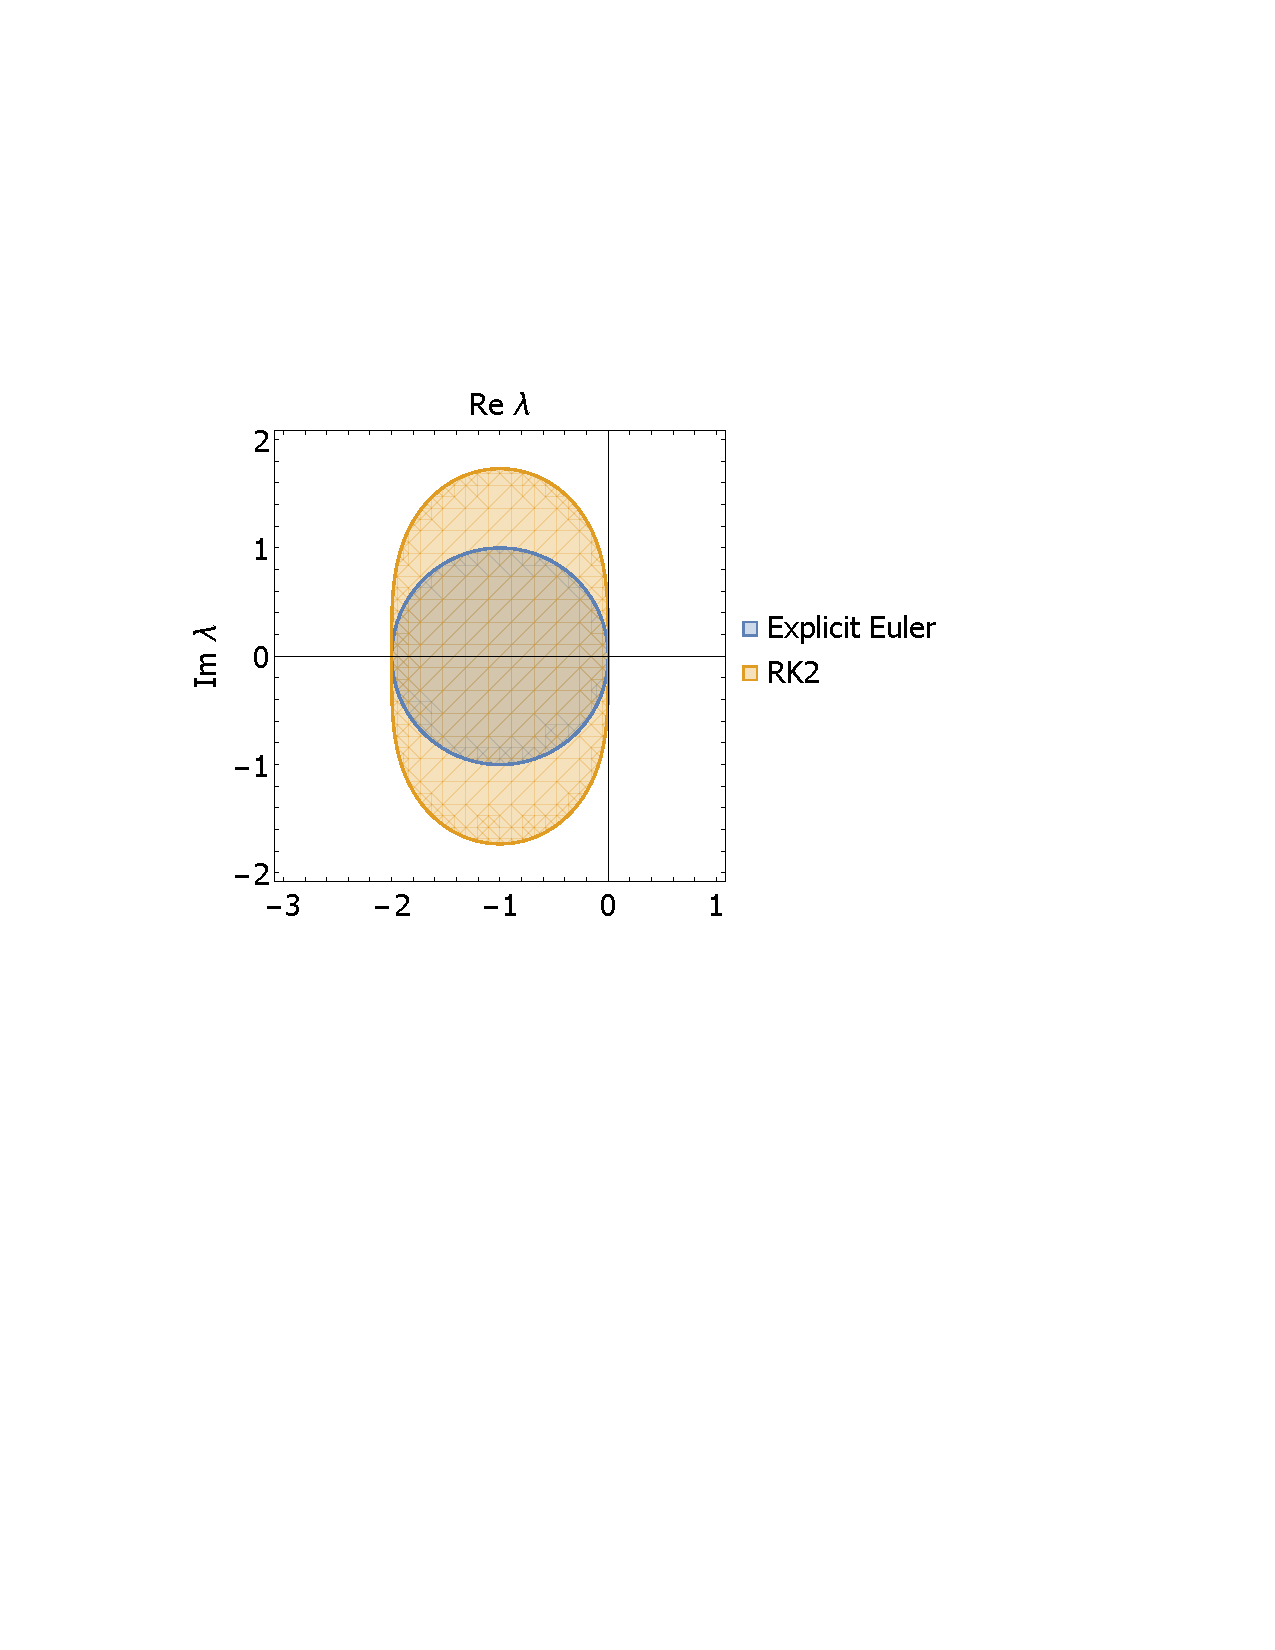
\includegraphics[scale=0.65]{figures/fig_stability_RK_Euler.pdf}
    \end{center}
  \caption{Stability regions of the explicit Euler and RK2 methods. }
  \label{fig_stability_RK_Euler}
\end{figure}
As we show in Figure~\ref{fig_stability_RK_Euler}, the stability region for the RK2 method is slightly larger in the imaginary direction than the explicit Euler \cite{griffiths_numerical_2010}. For advection-dominated problems, the spread of the eigenvalues of the Jacobian matrix is mostly along the imaginary direction. For this reason, we expect better stability for our problem as the diffusion is small compared to the advection. 
\par
As we are concerned with the stability of explicit schemes, it would be useful to have an implicit time integration for the second-order strain tensor flow. Although further investigation is necessary, we anticipate having a second-order convergence with better stability with the following predictor-corrector scheme \cite{press_numerical_2007},
\[
{\color{blue}\vec{u}^{temp}} -
\frac{1}{\rho} \nabla
\left( 
\frac{\nabla \cdot {\color{blue}{\bm \tau}_1^{temp}}}{2}
\right)
=
\vec{u}^n
+ \tilde{\bm F} \left( \vec{u}^{n} \right) \Delta t
+ \frac{1}{\rho} \nabla \biggl(
\frac{ \nabla \cdot{\bm \tau}_1^n}{2} 
+ \nabla \cdot {\bm \tau}_2^n 
\biggr)\Delta t
\]
\[
{\color{red}\vec{u}^{n+1}} 
- \frac{1}{\rho}\nabla 
\left(
\frac{\nabla \cdot {\color{red}{\bm \tau}_1^{n+1}}}{2}
\right)
=
\vec{u}^n 
+ \tilde{\bm F} \left( \vec{u}^{n} \right) \Delta t
+ \frac{1}{\rho} \nabla \biggl(
\frac{ \nabla \cdot{\bm \tau}_1^n}{2} 
+ \frac{\nabla \cdot {\bm \tau}_2^{n} + \nabla \cdot {\color{blue}{\bm \tau}_2^{temp}}}{2} 
\biggr)\Delta t
\] 
where 
\[
  \tilde{\bm F} \left( \vec{u}^{n} \right)= 
    -\vec{u}^n \cdot \nabla \vec{u}^n 
    +\frac{1}{\rho}
    \biggl(
    - \nabla P^n 
        % + \nabla \cdot   \bm{\tau}(\vec{u}^n)
        +  \rho  \vec{g} 
        \biggr).
\]
The idea is similar to an implicit RK2 scheme. The main difference is that we split the viscous tensor $\bm \tau$ term into two parts,
\[
{\bm \tau_1} \propto {\bm D}, \ \ \ {\text{and}} \ \ \  {\bm \tau_2} \propto {\bm D^2}.
\]
The complication of this implementation is building the linear system to solve for each velocity, $\vec{u}^{temp}$ and $\vec{u^{n+1}}$. 
% This requires a deeper understanding and knowledge of the main AMReX library. 
%If we have more advection dominant flow than diffusion, it is possible to have all imaginary eigenvalues of the Jacobian of the right-hand side of equations~(\ref{eq_RK2_s1}) and~(\ref{eq_RK2_s2}). In that case, we might be able to use a bigger time step size than the explicit Euler. 
\par
From the second-order strain rate rheology perspective, we consider adding the time-dependent term, 
\begin{equation}
  % \bm{\tau} =  \mu_1 {\bm D} 
  %   + \mu_2  \left[ {\bm D}^2  - \frac{\text{tr}\left({\bm D}^2\right)}{3}{\bm I} \right]
  %  + \kappa_1 \frac{{\bm D}}{|{\bm D}|} 
  %   + \kappa_2  \left[ \frac{{\bm D}^2}{|{\bm D}|^2}  
  %   - \frac{\text{tr}\left({\bm D}^2\right)}{3|{\bm D}|^2}{\bm I} \right]
  %   + 
  \mu_3  \left[ {\bm D}{\bm W} - {\bm W}{\bm D},\right]
  \end{equation}
  to the stress tensor give in equation~(\ref{eq_2ndOrder_tau}).
 The viscosity coefficient can be found by modifying the $\mu(I)$ rheology~(\ref{eq_muI_general}),
\begin{equation}
    \mu(I)_3 = -A_3 \left( I^2 \right)^{\alpha_3} = \frac{\eta_3 \dot{\gamma}^2}{P}.
\label{eq_muI3}
\end{equation}
Specifically, we can find the coefficients of each shear rate term in equation~(\ref{eq_2ndOrder_tau}) as
\begin{equation}
     \mu_3  = 
    - P A_3 
        \left( \frac{\dot{\gamma} d }{\sqrt{P /\rho}}  \right)^{2\alpha_3} 
        \frac{1}{\dot{\gamma}^2}.
\label{eq_gr_eta_3}
\end{equation}
To obtain more realistic simulations, it would be necessary to connect the granular rheology with a compressible flow.
\par
It is also interesting that solid particles suspended in a Newtonian fluid can exhibit highly non-Newtonian behaviors. To model this type of behavior, we may implement immersed boundary methods to simulate a suspension of solid particles in a Newtonian fluid, which is an important application area that has received significant research interest lately~\cite{couturier_suspensions_2011}.
% \par 
% In addition to granular material for industrial and natural significance, I personally am interested in studying biofluids as an extension of this complex fluid project. According to~\cite{xue_modelling_2011}, 
\begin{comment}
\par
Add surface tension effect in AMReX-incflo. 
\par
This section summarizes the rheological model of suspensions in a Newtonian fluid. Solid particles suspended in a Newtonian fluid can exhibit highly non-Newtonian behaviors.  
\par
We use the constitutive equation proposed by Reiner \cite{reiner_mathematical_1945} and Rivlin \cite{rivlin_stress-deformation_1955},  
\begin{equation}
  \bar{\bar{\sigma}} = -P \bar{\bar{I}}
  + 2 \nu_1 {\bm{D}} + 2 \nu_2 {\bm{D}}^2.
\end{equation}
According to Tanner's review \cite{tanner_review_2018}, the coefficients $\nu_1$ can be constant since the rate of change with $\dot{\gamma}$ is negligible, and $\nu_2 = \beta / \dot{\gamma}$ for a suspension of solid particles in a Newtonian fluid, where a factor $\beta$ is related to the strain rate $\dot{\gamma}$. Dai et, al \cite{dai_viscometric_2013} shows the $\beta = -4.4 \phi^3 \nu_1$ in shear flows, where $\phi$ is a volume fraction. 
\end{comment}
